\chapter{System Design, Implementation, and Experimental Setup}\label{ch:system-design}

\hyperref[ch:related-work]{Chapter~3} showed that prior research typically treats semantic latent-space navigation, interactive exploration interfaces, and evaluation methods as largely separate areas. Comparatively little work combines reproducible tooling, graph-based exploration, and structured empirical analysis within a single workflow. This chapter presents the system developed to address that gap and describes the components of the exploration environment that were designed and implemented specifically for this thesis, based on the concepts introduced in \hyperref[ch:foundations]{Chapter~2}.

\section{Requirements for the exploration environment}\label{sec:4.1}

The gap identified above, leads to four requirements for the exploration environment. First, prompt datasets and their compact embeddings must be created and extended through a reproducible process without requiring manual data management. This ensures that the empirical analyses presented in later chapters are based on a consistent and traceable dataset foundation. Second, the resulting embeddings must support projection and clustering, and both the resulting structure and the outputs of navigation operations must be available for interactive inspection rather than only as static results. Third, the environment must provide multiple navigation methods, including interpolation and direction-based movement, with explicitly defined and recorded parameters. Their outputs must remain traceable to the source points and settings from which they were generated. Fourth, the implementation must neither modify the diffusion model's architecture nor the ComfyUI core. Navigation results must also be transferable back into ComfyUI's standard image-generation pipeline so that they can be rendered as images rather than examined only as numerical representations.

The remainder of this chapter addresses these requirements. \hyperref[sec:4.2]{Sections~4.2} and \hyperref[sec:4.3]{4.3} introduce the selected technologies and component architecture, primarily addressing the fourth requirement, while also touching on the interactive-inspection part of the second requirement. \hyperref[sec:4.4]{Section~4.4} presents a deeper understanding of the interaction design derived from the second and third requirements. \hyperref[sec:4.5]{Section~4.5} defines the model, encoder, and prompt sources used throughout the thesis. \hyperref[sec:4.6]{Section~4.6} describes the dataset-construction pipeline, including prompt acquisition, encoding, projection, clustering, and storage, thereby addressing the first and second requirements. \hyperref[sec:4.7]{Section~4.7} explains the runtime session architecture that connects the frontend and backend. \hyperref[sec:4.8]{Section~4.8} introduces the navigation operations and their integration into the image-generation workflow, addressing the third and fourth requirements. Finally, \hyperref[sec:4.9]{Section~4.9} discusses the resulting design trade-offs and the validity limitations of the implementation.

\section{Technology and platform selection}\label{sec:4.2}

Two requirements identified in the previous section directly influence the technological and platform decisions made in this work. First, the plugin must integrate with ComfyUI's existing image-generation pipeline without retraining the underlying model or modifying ComfyUI's core. Second, it must support interactive exploration of embeddings and navigation results rather than providing only static visualizations. To meet these requirements, Python, TypeScript, ComfyUI, and the supporting libraries were adopted and used as existing technologies.

ComfyUI was selected as the host platform because this thesis examines the latent space of an existing diffusion model rather than introducing a new generative architecture. The open source platform is described by its maintainers as "The most powerful and modular diffusion model GUI, api and backend with a graph/nodes interface" \cite{comfyorg2026github}. During the evaluation process, its codebase was examined with the assistance of DeepWiki, an AI-supported tool for exploring software repositories \cite{deepwiki2026tool}. A representative example of this tool interaction is provided in \hyperref[app:1-comfyui]{Appendix 1}.
A central selection criterion was the availability of a complete image-generation pipeline. The chosen platform needed to provide model loading, conditioning, and sampling functionality so that the implementation could focus on latent-space navigation and analysis rather than reproducing established generation infrastructure. ComfyUI satisfies this requirement and also provides an extension mechanism through which custom nodes and frontend components can be added without modifying its core source code \cite{comfyorg2026overview}. This allows navigation results to be integrated directly into the same pipeline that ultimately converts them into generated images.
ComfyUI also provides an established environment in which the resulting plugin can potentially remain usable and extensible beyond the scope of this thesis. Alternative approaches, including a standalone application with a separate generation backend or integration into another web interface, were considered but not pursued. Both would have required duplicating actively maintained generation functionality without providing a clear advantage for the navigation and analysis methods investigated in this work.

ComfyUI is available in several distribution formats. The Desktop application provides a launcher for managing one or more ComfyUI installations \cite{comfyorg2026desktop}, while the portable distribution is a self-contained package that includes its own Python environment and can be extracted and executed directly \cite{comfyorg2026portable}. A hosted cloud version is also available, but it is not considered in this thesis because the implementation and testing of the plugin require access to a local extension environment.

Development was carried out on Windows using the portable distribution. This setup provides the needed direct access to the filesystem and, in particular, to the \texttt{custom\_nodes} directory in which the plugin is installed. The underlying user interface remains the same across the Desktop and portable distributions, but it is presented differently. In the Desktop application, the web interface is embedded within the application window. In the portable setup used for this project, ComfyUI runs as a local web server, and the interface is opened separately in the user's browser through localhost.

Python is used as the primary backend language because ComfyUI's node-execution system is implemented in Python \cite{comfyorg2026walkthrough}. Implementing the encoding, dataset construction, projection, clustering, and navigation operations in the same language allows the plugin to integrate directly with ComfyUI and it allows the use of PyTorch for tensor-based computation. It also provides access to the Python-based machine-learning ecosystem required by the projection and clustering methods introduced in \hyperref[ch:foundations]{Chapter~2}. The implementation further relies on Hugging Face's \texttt{datasets} library for loading prompt corpora and on \texttt{transformers} for language models used during cluster annotation \cite{huggingface2026datasets,huggingface2026transformers}.

For the interactive frontend, TypeScript was selected because ComfyUI's extension mechanism for custom panels and widgets is based on JavaScript and TypeScript. The source code is compiled with Vite into a JavaScript bundle that can be loaded by the browser.
Plain JavaScript was considered as an alternative but rejected because the graph panel manages increasingly complex states, including selected nodes and points, trajectory settings, operation parameters, and data exchanged between the frontend and backend. TypeScript's static type checking helps detect inconsistencies in these data structures during development and reduces the risk of state-management and interface errors as the frontend evolves.

Together, these three technology choices satisfy the requirement of integrating the exploration environment directly into an existing and unmodified image-generation system while also providing an interactive interface for inspecting embeddings and navigation results.

\section{NeLs: an external ComfyUI plugin}\label{sec:4.3}

The previous section established that NELS can be integrated into ComfyUI through its extension system without modifying the ComfyUI core. This section describes how the plugin implements this integration and how its internal components are organized.

ComfyUI discovers custom nodes by scanning the \texttt{custom\_nodes} directory noted above for Python modules that expose a \texttt{NODE\_CLASS\_MAPPINGS} dictionary. When a module is imported successfully and provides this mapping, the registered classes become available as nodes in the workflow editor \cite{comfyorg2026lifecycle}. NELS follows this convention in its top-level initialization module. The module collects the node classes defined throughout the plugin into a single mapping, registers the HTTP routes required for session management, and exposes the directory containing the frontend assets through \texttt{WEB\_DIRECTORY} \cite{comfyorg2026lifecycle}.
As a result, the complete plugin can be installed within a single directory under \texttt{custom\_nodes} and is discovered automatically when ComfyUI starts. No modification of the ComfyUI source code is required.

Below this entry point, the implementation is divided into five components with distinct responsibilities:

\begin{itemize}
\item \textbf{\texttt{nodes/}} contains the classes exposed directly in the ComfyUI workflow editor. These classes define the required input and output interfaces for components such as dataset loading, session handling, and graph operations. They remain intentionally thin and delegate the underlying computation to the reusable implementation in \texttt{core/}. From the user's perspective, the classes in this directory behave like standard ComfyUI nodes and can be connected and executed within an ordinary workflow.
\item \textbf{\texttt{core/}} contains the main computational and semantic logic of the plugin. This includes prompt encoding, dataset construction, projection and clustering, and the six operation families introduced in \hyperref[sec:4.8]{Section~4.8}. The code is implemented as ordinary Python functionalities and does not depend on being executed through a ComfyUI node. This separation allows the computational logic to be tested and reused independently of the ComfyUI runtime.
\item \textbf{\texttt{server/}} provides the connection between the frontend and the backend session state. It defines the required HTTP routes and maintains an in-memory session store within ComfyUI's existing server process rather than starting a separate server. This additional communication layer is necessary because the graph panel requires continuous interaction between the browser and the backend beyond the input-output flow of a single node execution. ComfyUI categorizes this type of extension as a connected client-server integration \cite{comfyorg2026overview}.
\item \textbf{\texttt{src/}} contains the interactive graph-panel frontend, implemented in TypeScript and Preact. Vite compiles these sources into the JavaScript files loaded by the ComfyUI client. The frontend architecture and its interaction model are discussed further in \hyperref[sec:4.4]{Sections~4.4} and \hyperref[sec:4.7]{4.7}.
\item \textbf{\texttt{scripts/}} provides command-line entry points for offline processing. These scripts access the functionality in \texttt{core/} directly and do not depend on the node definitions, session server, or a running ComfyUI web client, though they still import ComfyUI's own model-loading and CLIP-encoding classes directly, so a ComfyUI installation must still be present on the machine running them. They are primarily used for batch dataset creation and related preprocessing tasks.
\end{itemize}

This separation supports the architecture required by Requirement 4. Only the node and server layers interact directly with ComfyUI-specific interfaces, while the central computation remains isolated in a reusable core.

The client-server architecture also introduces a practical limitation. According to the ComfyUI documentation, extensions that depend on direct communication between the browser client and the server are not compatible with ComfyUI's plain API mode \cite{comfyorg2026overview}. The interactive graph panel therefore requires the standard ComfyUI web client. While individual server-side nodes may be executed headlessly, interactions such as point selection, operation configuration, and live graph updates cannot be controlled solely through the API.

\section{UI/UX design rationale}\label{sec:4.4}

This section discusses two central UI/UX design decisions and the interaction features that result from them: first, why the exploration interface is embedded directly within ComfyUI rather than implemented as a separate application, and second, why the dataset is presented as an interactive graph instead of through a form- or table-based interface.

Embedding the panel within ComfyUI follows directly from Requirement 4 and the architecture described in \hyperref[sec:4.3]{Section~4.3}. Since the results of the navigation process must be transferred back into ComfyUI's standard image-generation workflow, placing the exploration interface alongside the node graph avoids switching between a separate analysis tool and the generation environment. The panel is implemented with Preact \cite{preactjs2026core}, a lightweight alternative to React that provides a similar component model and broad compatibility with the React API, together with \texttt{@preact/signals} \cite{preactjs2026signals}, a library for reactive state management. It provides separate graph and log views, while a resizable sidebar contains the operation controls, results, and session information. The selected sidebar width is preserved between sessions, allowing the interface to adapt to different tasks without introducing unnecessary interface elements.

The dedicated panel was not the initial interface design. ComfyUI also supports custom widgets rendered directly within a node on the workflow canvas, and this in-node approach was first considered because it would have integrated the exploration interface even more closely with the graph workflow. However, it became unsuitable as the performance and interaction requirements expanded. Displaying a live graph containing hundreds or thousands of points, together with panning, zooming, hovering, multi-selection, drag selection, and point-specific context actions, proved impractical within the limited dimensions, layout constraints, and event-handling environment of a single node. Once the full scope of the required interaction became clear, a dedicated panel offered the more appropriate solution by providing independent screen space, flexible resizing, and event handling separate from the node-graph canvas.

The graph-based interaction model was inspired by GitNexus, a tool that represents the structure of a codebase as a navigable knowledge graph of related code entities \cite{patwari2026gitnexus}. No source code or interface components from GitNexus were reused. Only the broader interaction concept of exploring a large structured space through spatial relationships rather than by scrolling through a linear list was adopted. Before implementing this approach, the GitNexus codebase was examined with the support of DeepWiki. A representative example of this tool interaction is provided in \hyperref[app:1-gitnexus]{Appendix 1}. In NELS, the points represent prompts and their embeddings rather than code entities, but the underlying interaction problem remains comparable: users must navigate a large collection of related items through their spatial proximity and connections.

Since the dataset can be projected into either 2 or 3 dimensions, the panel provides both a two-dimensional and a three-dimensional graph view. The 2D view is implemented with Sigma.js \cite{jacomy2024sigmajs}, a WebGL library for rendering large graphs in the browser, together with Graphology \cite{plique2021graphology} for the underlying graph data structure, while the 3D view is built with Three.js \cite{threejs2026}, a general-purpose library for rendering 3D scenes in the browser. Despite relying on different rendering technologies, both views use the same interaction model. Clicking selects a point, modifier-assisted clicking extends the current selection, and shift-dragging creates a selection area that includes all enclosed points. Hovering displays a tooltip with the corresponding point information, while right-clicking opens a contextual action menu. Maintaining the same interaction vocabulary across both views ensures that switching between 2 and 3 dimensions changes only the visual representation, not the way the user operates the interface.

Operation outputs are integrated directly into the existing graph rather than presented in a separate results view. Trajectory steps produced by interpolation or direction-based operations, as well as variant points generated by the Consistency Check, appear alongside the original dataset points. They are distinguished visually through a different texture, a highlight ring, and a subtle animation, but otherwise support the same interactions. This includes selection, hovering, and context-menu actions. Internally, these temporary points are identified through a dedicated prefix.

Two additional interface elements support interpretation of the displayed structure. The cluster legend lists each detected cluster together with a color indicator, a representative prompt, and the number of associated points. Selecting a legend entry emphasizes the corresponding cluster while dimming the remaining graph. The legend can also report how many generated result points are assigned to a cluster, even when none of that cluster's original samples are included in the currently loaded subset. For Semantic Axis Projection, a separate axis legend displays the human-readable labels of both semantic poles alongside the numerical projection score. This ensures that the resulting values remain connected to their intended semantic interpretation.

The panel includes a purely cosmetic idle animation, namely a subtle and continuous jitter of point positions, so that the graph does not look static and users are encouraged to interact with it rather than treat it as a passive tool. This choice comes with a deliberate limitation: when animation is enabled, points move smoothly between states, but the intermediate positions shown during this movement are not geometrically exact. The interface communicates this limitation explicitly through the notice "animate ON - positions not exact," reducing the risk that a visually smooth transition is interpreted as a precise trajectory.

The resulting interface prioritizes functional interactivity and a consistent interaction model over visual refinement, as shown in \hyperref[fig:panel-ui-2d]{Figure~\ref*{fig:panel-ui-2d}} and \hyperref[fig:panel-ui-3d]{Figure~\ref*{fig:panel-ui-3d}}. Since it was developed as a research prototype for investigating latent-space navigation rather than as a production-ready application, its visual design and overall interface polish were not prioritized and remain open for future improvement.

To conclude this section, the frontend was developed with the assistance of Claude Code using the Claude Sonnet 4.6 model. Development was guided by a written specification file that defined the intended architecture, components, and interaction behavior. Individual implementation details were then refined iteratively through follow-up prompts. The specification is included in \hyperref[app:2]{Appendix 2} to document and support the development process.

\begin{figure}[htbp]
\centering
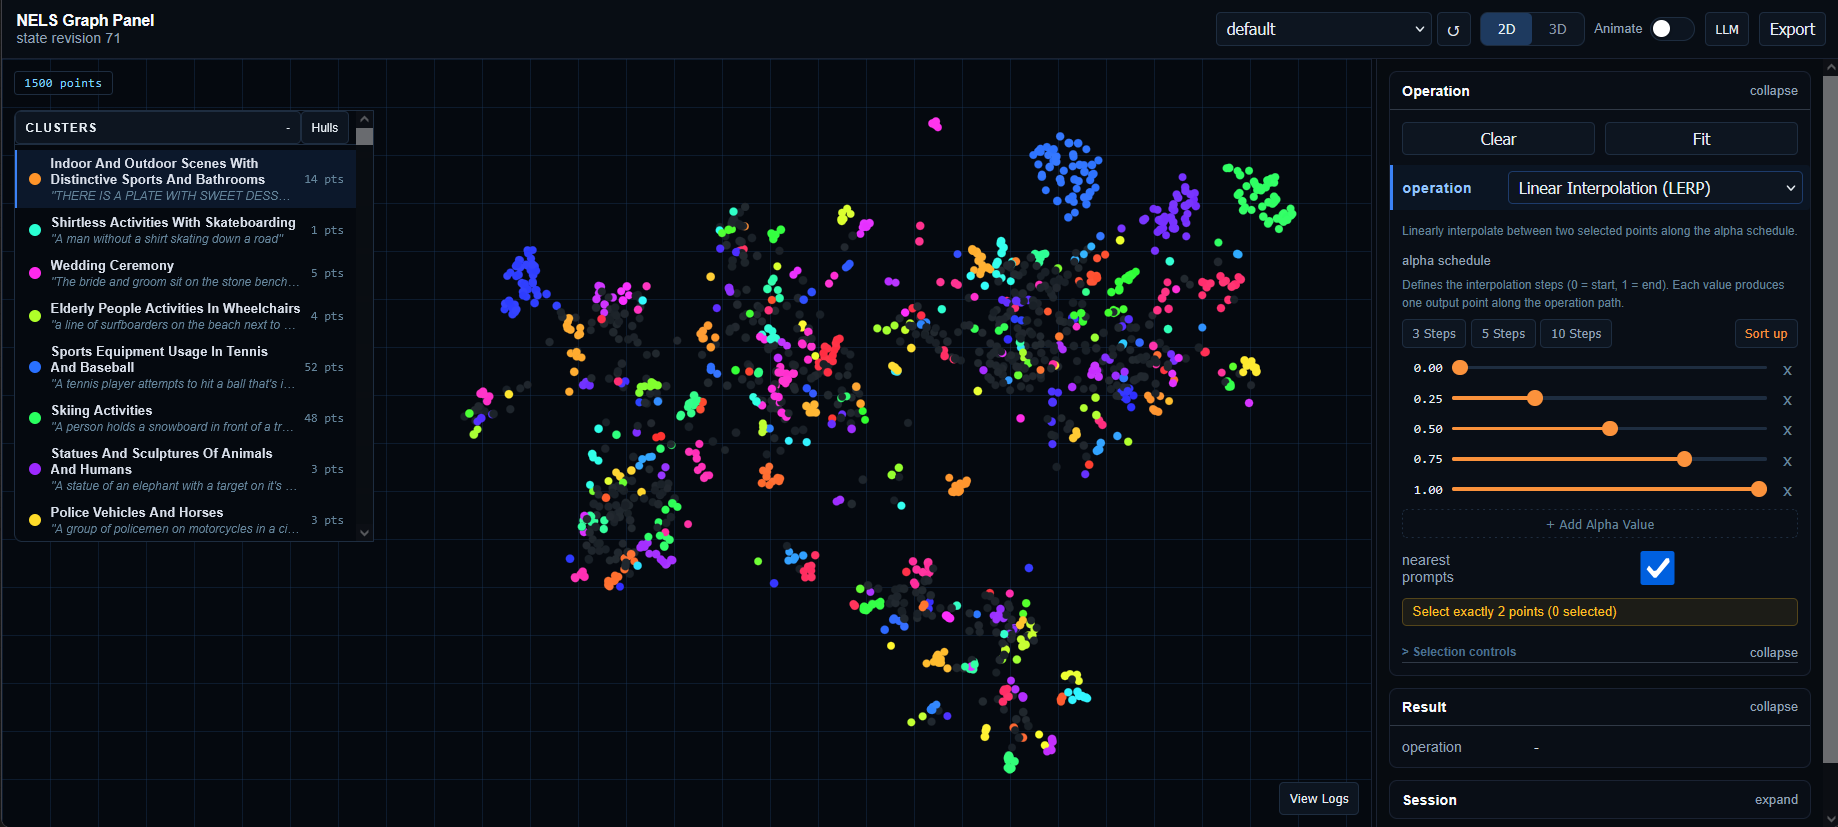
\includegraphics[width=0.82\textwidth]{figures/panel-ui-2d.png}
\caption{The NELS graph panel in 2D view: 1500 points colored by cluster, the cluster sidebar with legend, and the operation controls}
\label{fig:panel-ui-2d}
\end{figure}

\begin{figure}[htbp]
\centering
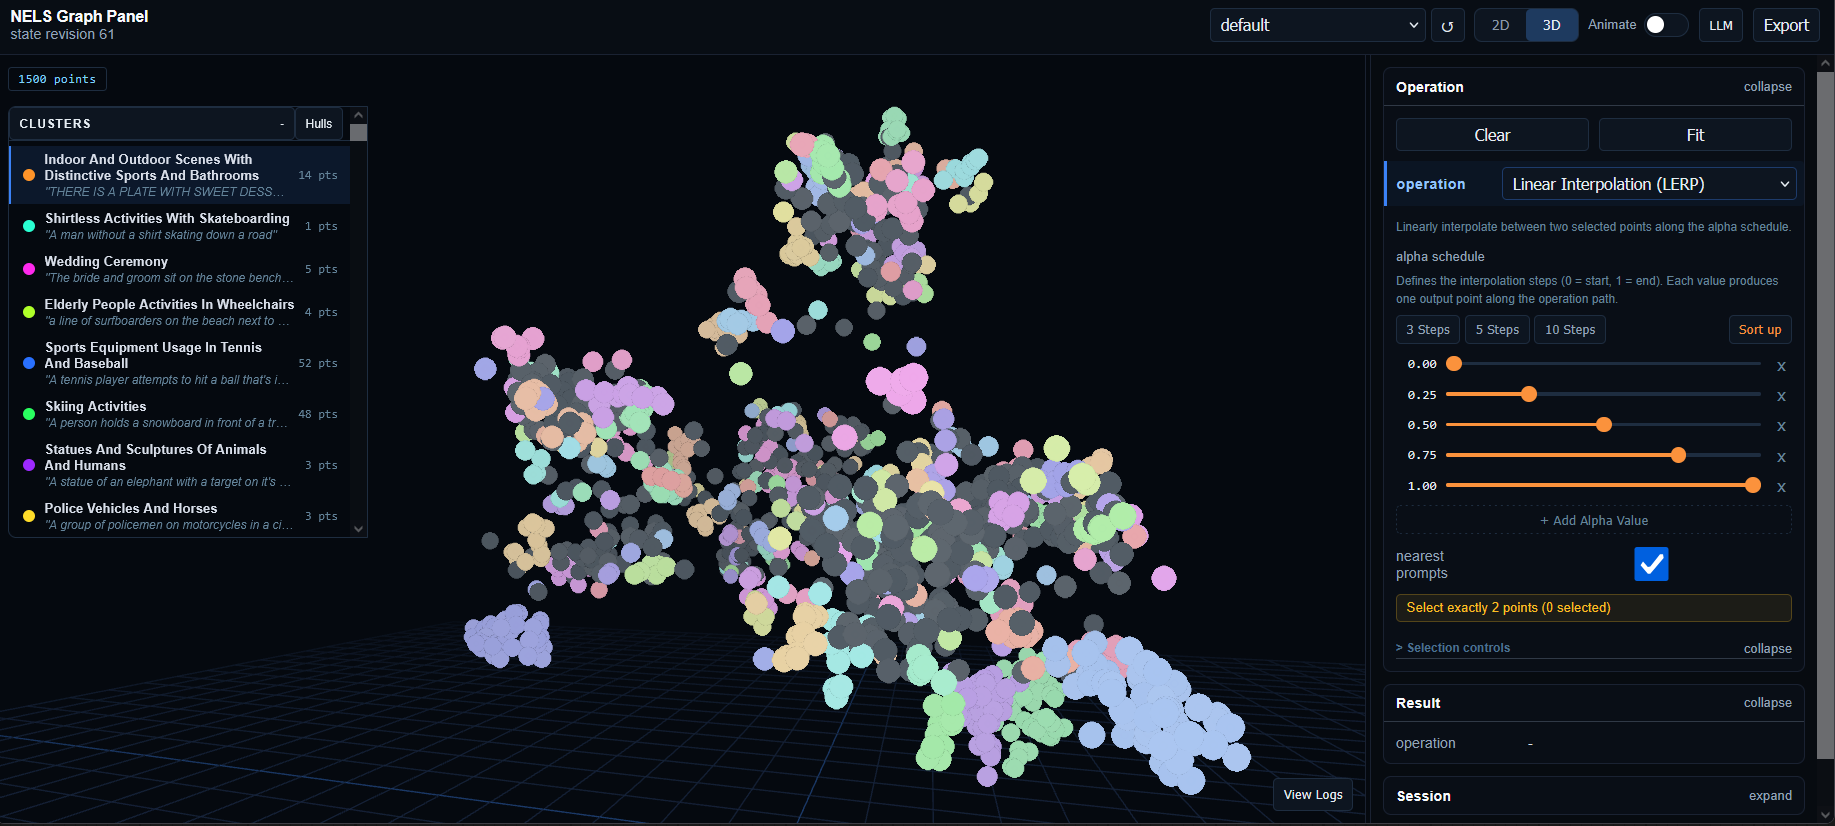
\includegraphics[width=0.82\textwidth]{figures/panel-ui-3d.png}
\caption{The same session in 3D view}
\label{fig:panel-ui-3d}
\end{figure}
\FloatBarrier

\section{Model, encoder, and prompt-source selection}\label{sec:4.5}

Having described how the panel presents results and supports user interaction, the following section introduces the model, encoder, and dataset choices that determine the content displayed within it. All experiments in this thesis use Flux.2 Klein, an open-weight rectified-flow model with approximately four billion parameters that supports both text-to-image generation and image editing. Text conditioning is provided by its associated Qwen-based encoder \cite{blackforestlabs2026flux2klein}. Both components are loaded through ComfyUI-compatible \texttt{.safetensors} conversions distributed by the ComfyUI community \cite{comfyorg2026hfmodels}.

The availability of open weights was the primary selection criteria for the models, because the investigation requires local access to the model and the ability to inspect and repeatedly execute it without relying on a closed external API. At the beginning of the implementation period, Flux.2 Klein was selected as the most suitable open-weight model available for these requirements. Since the field develops rapidly, however, newer and more capable open-weight models may become available after the publication of this thesis.

Both the diffusion model and the text encoder are used in quantized form: FP8 (8-bit floating point) for the diffusion model and FP4 (4-bit floating point) for the encoder, which reduces both memory usage and compute during inference. This configuration was selected because it could be executed reliably on the available hardware, namely an NVIDIA GeForce RTX 2070 with 8 GB of VRAM, paired with an AMD Ryzen 5 3600 6-core processor and 32 GB of system RAM. Full-precision checkpoints would have been preferred if sufficient computational resources had been available. Quantization may influence the precise numerical properties of the representations examined in later chapters, although it is not expected to fundamentally alter the qualitative structures investigated in this thesis.

The datasets examined in this thesis comprise four large prompt corpora representing two qualitatively different text distributions, complemented by a small controlled label set for comparing projection strategies. Natural image-caption prompts are drawn from CaptionEmporium's LLaVA-generated short captions for Conceptual Captions CC12M \cite{captionemporium2026cc12mllavanext}, a large-scale corpus of web-sourced image-text pairs \cite{changpinyo2021cc12m}, and from COCO Captions \cite{jxie2026cococaptions}. Prompts that more closely resemble the descriptive, "AI-art"-style input commonly used in text-to-image systems are taken from daspartho's Stable Diffusion Prompts dataset \cite{daspartho2026sdprompts} and Gustavosta's Stable Diffusion Prompts dataset \cite{gustavosta2026sdprompts}. Including both distributions makes it possible to examine whether the observed navigation behavior remains consistent across different forms of prompt language rather than being specific to a single writing style.
A fifth, much smaller dataset is also used: the 1.000 ImageNet-1k class labels \cite{ilsvrc2026imagenet1k}, selected because they provide a compact, clearly defined, and well-understood label set for the projection-strategy comparison described in \hyperref[sec:4.6]{Section~4.6}, in contrast to the long and heterogeneous natural-language prompts of the four corpora above.

The ImageNet labels were not initially prepared through the pipeline's generic Hugging Face input mechanism because the dataset's label column stores each class as an integer index, through a \texttt{ClassLabel} feature, rather than as usable text. The generic loader has no step to resolve that index into its corresponding class name. Instead, a one-off preprocessing script streamed the training split of the ImageNet-1k dataset through the Hugging Face \texttt{datasets} library and retrieved the decoded class names from the label feature's list of class names rather than using the stored integer indices. Each class name was then converted into a prompt of the form "a photo of \{name\}" and written to a local text file containing one prompt per line. This file was subsequently processed through the pipeline's standard local-file input path.

As described in the next section, the dataset-construction pipeline treats prompt sources generically rather than being tied to any specific corpus. Combined with the separation between the node interface and the underlying processing logic discussed in \hyperref[sec:4.3]{Section~4.3}, this design allows both the prompt source and the model implementation to be exchanged without restructuring the pipeline. The same construction and analysis workflow could therefore be applied to all four large corpora and to the differently formatted ImageNet label file.

\section{Data acquisition and processing}\label{sec:4.6}

This section describes the dataset-construction pipeline, including how the plugin collects prompts, encodes and compacts them, projects and clusters the resulting representations, stores the dataset, extends it at a later stage, and assigns labels. The subsection concludes by differentiating between the two representation spaces on which the pipeline operates.

A dataset can be created either through the prompt-encoding node or through the corresponding command-line interface, which executes the same processing pipeline without requiring an active ComfyUI session. Both paths intentionally use the same ComfyUI-native model classes and compatible model weights. As a result, they produce byte-for-byte identical compact embeddings.
Using the original model release instead would not affect projection, clustering, or interpolation, since these operations work only with vector representations, but the resulting incompatibility would only become noticeable during image generation. At that stage, the original model's conditioning tensors would not match the shape and conventions expected by ComfyUI's sampling pipeline, preventing the generated conditioning from being processed correctly. Using the ComfyUI-compatible model implementation during dataset construction therefore ensures that every dataset remains compatible with the later image-generation pipeline.

Prompt records are first collected into a single ordered list from as many as two sources: text entered directly in the node and an optional external source. The external input may be either a local text file containing one prompt per line or a streamed Hugging Face dataset selected by repository, split, and configuration where required, optionally combined with a template that merges dataset columns into the prompt text and copies additional metadata into each record.
The collected records are then cleaned, filtered by minimum and maximum word count, and optionally deduplicated. Because the external source is capped before deduplication, enabling it can yield fewer records than requested. The final size limit, applied after merging inline and external, then trims excess from the external records first, since inline prompts are retained preferentially.

Each prompt record is encoded exactly once. Tokenization first converts the prompt into a token sequence, after which a single encoder forward pass returns the full sequence-conditioning tensor and, where supported, a pooled representation. From these outputs, one fixed-size compact vector is derived and stored for the prompt. If a pooled representation is available, it is converted to floating-point format. If it is not already one-dimensional, its leading dimension is removed to produce a one-dimensional vector. For example, a pooled output with shape \texttt{[1, D]} becomes a vector of shape \texttt{[D]}. If no pooled representation is available, the leading batch dimension of the sequence tensor is removed and the remaining token vectors are averaged:
\[
e_{\text{prompt}} = \frac{1}{n} \sum_{i=1}^{n} e_i,
\]
where $n$ is the number of token positions and $e_i$ is the representation of the $i$-th token.

The Qwen-based encoder used throughout this thesis does not provide a pooled output. Consequently, all datasets created for this work use mean pooling over the sequence and record this fallback strategy in their metadata as \texttt{embedding\_strategy: mean\_seq\_fallback}. The pooled-output branch remains available for other encoders but is not used by any dataset evaluated here. Mean pooling was chosen for its fixed-size, length-independent representation that lets every token position contribute to the representation, though it is treated as a weaker representation than a dedicated pooling head.

For the encoder described in \hyperref[sec:4.5]{Section~4.5}, the full conditioning tensor of a single prompt has shape \texttt{[1, 512, 7680]}, corresponding to 512 token positions with 7.680 features each. Stored as 32-bit floating-point values, this requires roughly 16 MB per prompt and approximately 8 TB for a dataset of about 550.000 prompts. The corresponding compact representation has shape \texttt{[7680]}, requires roughly 31 KB per prompt, and occupies approximately 16 GB for the same dataset size. The storage requirement is therefore reduced by a factor of exactly 512, corresponding to the number of token positions collapsed into one vector. This reduction is why dimensionality reduction, clustering, and nearest-neighbor search operate on the compact vectors rather than the full conditioning tensor.

The current pipeline processes prompts sequentially, using one encoder forward pass per prompt since pooled representations are requested individually, and requires every prompt in a dataset to use the same representation strategy. Encoding is stopped with an explicit error if some prompts would use native pooling while others require mean pooling, preventing incompatible representations from being silently combined in the same embedding matrix. This situation does not arise in practice, since pooling availability is a property of the encoder rather than of individual prompts and a dataset build always uses one encoder.

Finally, sample identifiers are assigned in ascending order during dataset creation, ensuring that they remain stable and searchable across later operations.
The dataset's metadata, saved into \texttt{dataset.json}, describes both how the dataset was built and what its clustering labels are. Saved information includes prompt source, template, and metadata columns used to build the dataset, the encoder and model used to produce the compact vectors, and the projection strategy and umap parameters used to produce the two- and three-dimensional coordinates as well as how the clusters get computed. This metadata is used to inspect the dataset's construction and to ensure that it can be rebuilt or extended later with the same parameters.

Once compact vectors have been generated for all prompts, the resulting embedding matrix is used to train the projection models. Separate UMAP models are fitted for the two- and three-dimensional views displayed in the graph panel. Both models operate on the same complete compact embedding matrix and use the same UMAP parameter settings stored in the dataset metadata.
Fitting the model to the data and computing the display coordinates for the existing samples happen together. The resulting coordinates are stored as static arrays and later used to render the dataset. The fitted UMAP models are retained separately so that they can subsequently project new points and operation trajectories into the same coordinate spaces. How these reusable projection models are stored and applied depends on the selected projection strategy, described later in this section.

Cluster assignment is performed neither in the two- or three-dimensional display space nor directly in the full compact embedding space. HDBSCAN identifies clusters by estimating local density from pairwise distances. In the original 7.680-dimensional space, however, distances tend to concentrate: the relative difference between a point's nearest and farthest neighbors decreases as dimensionality increases, making density estimates less reliable \cite{aggarwal2001distancemetrics}. Density-based clustering methods such as HDBSCAN are therefore also affected by the challenges of high-dimensional data in practice \cite{mcinnes2026umapclustering}.
To address this issue, a third UMAP model is fitted specifically for clustering. Unlike the display projections, which reduce the embeddings to 2 or 3 dimensions, this model reduces them only to a moderate dimensionality, between 10 and 20 components for the datasets used in this thesis. This follows the recommendation in the UMAP documentation to preserve more cluster-relevant structure when dimensionality reduction is used as a preprocessing step for clustering \cite{mcinnes2026umapclustering}. The resulting coordinates form a separate cluster space that is used exclusively as the input to HDBSCAN.

HDBSCAN is then fitted on the reduced cluster-space coordinates using user defined cluster settings. Each point receives a cluster label, where a value of -1 denotes noise, together with a membership strength that reflects HDBSCAN's confidence in the assigned cluster. The clustering model is also configured to retain the information required for approximate prediction, allowing newly introduced points to be assigned to an existing cluster without refitting the complete model.

The clustering projection, the two display projections, and the HDBSCAN model are each fitted once on the complete dataset, in what NELS refers to as the canonical fit. This fit forms the fixed reference against which later runtime projections and cluster predictions are evaluated. How these fitted components are preserved and subsequently used to position and assign genuinely new points depends on the selected projection strategy, which is described in the following section.

The \texttt{classic} strategy stores the fitted cluster-space, two-dimensional, and three-dimensional UMAP models directly, together with the HDBSCAN clusterer, each serialized separately with \texttt{joblib} and reused at runtime. When new points must be displayed, the corresponding UMAP model transforms their compact embeddings into the previously learned projection space, yielding approximate coordinates since they are inferred rather than obtained by refitting UMAP with the new points included.
For cluster assignment, the new point is transformed into the learned cluster space and assigned via HDBSCAN's approximate prediction, which can only select among clusters from the canonical fit rather than create new ones. The \texttt{classic} strategy is the most direct and transparent of the three approaches, reusing the canonical fit's models unchanged rather than introducing a separate runtime approximation. Consequently, runtime projection depends on the fully fitted UMAP model, so transformation time and model size increase with the size of the original dataset, limiting the strategy's scalability.

The \texttt{parametric} strategy uses Parametric UMAP for the same three projection tasks: the two-dimensional display space, the three-dimensional display space, and the higher-dimensional cluster space. Instead of storing a non-parametric UMAP model, each projection is represented by a neural network trained with the TensorFlow/Keras backend introduced in \hyperref[sec:4.2]{Section~4.2}. The network learns a direct mapping from the compact embedding space to the respective target space.
Each trained projection is stored in a separate directory containing the neural encoder (\texttt{encoder.keras}) and the reducer's own saved state (\texttt{model.pkl}), while the HDBSCAN model is saved alongside them as \texttt{hdbscan\_model.joblib}. At runtime, new points are projected by passing their compact embeddings through the trained encoder. Cluster assignment follows the same principle as for the classic strategy.
The \texttt{parametric} strategy's main disadvantages are the additional dependencies and training complexity introduced by the Parametric UMAP and TensorFlow/Keras stack.

The \texttt{two\_pass} strategy is the most complex of the three: it performs the same canonical fit as the \texttt{classic} strategy, but once the cluster assignments and display coordinates have been produced, the fitted UMAP models are discarded rather than retained.
A second training stage then creates smaller projection models specifically for runtime use. By default, these models are fitted on a deterministically selected subset of 20.000 points and are stored separately for the two- and three-dimensional display spaces. The selected samples are also recorded to make the composition of the runtime subset inspectable. Rather than drawing a uniformly random sample from the whole dataset, the procedure ensures that each cluster identified during the canonical fit is represented in the subset in proportion to its size: a cluster that makes up, for instance, 10 percent of all clustered points also contributes about 10 percent of the subset. This also guarantees that even very small clusters contribute at least one point, which a purely random sample could otherwise skip entirely. If the proportional allocation cannot fill the requested subset size, the remaining slots are drawn from noise points instead. Within each cluster, points are sampled across the full range of membership strengths so that both strongly associated core points and weaker boundary points are represented.
New points are subsequently projected using these smaller runtime models instead of the discarded canonical models. Because they were fitted on only a subset of the complete dataset, they require less time and memory for transformation. The resulting coordinates are therefore a more approximate estimate of where the point would have been placed by the full canonical projection.

In the \texttt{two\_pass} strategy, cluster assignment for a newly introduced point is performed without using a cluster-space UMAP model. Instead, the operation builds a FAISS index over the complete compact embedding matrix and uses cosine similarity to retrieve the 32 most similar labeled samples. FAISS is a library designed for efficient similarity search in high-dimensional vector spaces \cite{douze2025faisslibrary}.

Their canonical cluster assignments are then combined through a temperature-scaled softmax vote. For the $i$-th of the $k = 32$ retrieved neighbors with cosine similarity $s_i$ to the new point, its vote weight is
\[
w_i = \frac{\exp(\tau \cdot s_i)}{\sum_{j=1}^{k} \exp(\tau \cdot s_j)},
\]
using a temperature of $\tau = 12$. Each neighbor's weight is added to the total weight of its own canonical cluster label, and the cluster with the greatest total weight is selected. The point is classified as noise when the winning label represents noise or when the winning label accounts for less than 45 percent of the total vote weight.

Several alternatives based on cluster-space projection were considered but rejected. One possibility was to project the new point through a hypothetical runtime UMAP cluster model and apply the canonical HDBSCAN model's approximate prediction function to the resulting coordinates. This approach would be invalid because the runtime cluster model and the canonical HDBSCAN cluster-space model were fitted independently and therefore do not represent the same manifold. As discussed in \hyperref[sec:2.4]{Section~2.4}, the geometry of a UMAP embedding depends on the data and configuration used during fitting. Consequently, the decision boundaries learned by the canonical HDBSCAN model cannot be transferred directly to coordinates produced by a separately fitted reducer.
A second alternative was to train a new cluster-space projection and HDBSCAN model on the same runtime subset. This was rejected for the same reason: a subset-trained projection would establish a different coordinate system and different cluster boundaries, causing predicted assignments to diverge from the canonical labels already stored with the dataset. A third possibility was to estimate the new point's canonical cluster-space position by averaging the cluster-space coordinates of its nearest neighbors and then applying approximate prediction. However, this would assume that proximity in the compact embedding space corresponds closely enough to proximity in the canonical cluster space for the averaged position to remain within the correct cluster.

The FAISS-based voting procedure avoids these problems by keeping the entire assignment process in the compact embedding space and combining neighbor labels rather than estimating an intermediate position. As a result, the \texttt{two\_pass} strategy uses two separate approximations: one determines where a new point is displayed, while the other independently estimates the canonical cluster to which it belongs.

Each completed dataset directory contains three core files: \texttt{dataset.json} (the metadata), \texttt{samples.jsonl} (the line-based sample file), and \texttt{compact\_embeddings.npy} (the full compact embedding matrix). Each entry in the sample file stores a prompt's identifier, text, source information, optional template or metadata fields, and its \texttt{cluster\_global}, \texttt{is\_noise}, and \texttt{membership\_strength} values.
The projection outputs take two fundamentally different forms. Static \texttt{umap\_2d.npy} and \texttt{umap\_3d.npy} coordinate arrays, generated when the dataset is created, hold the fixed positions of existing samples and are never transformed again. Serialized projection and clustering models are loaded only when genuinely new points must be projected or assigned to a cluster: \texttt{umap\_model\_2d}, \texttt{umap\_model\_3d}, and \texttt{umap\_model\_cluster} alongside \texttt{hdbscan\_model.joblib}, or the corresponding \texttt{runtime\_umap\_model\_2d.joblib} and \texttt{runtime\_umap\_model\_3d.joblib} used by the \texttt{two\_pass} strategy.

Beyond the coordinate arrays and projection models described above, every dataset also carries descriptive labels for its clusters, produced through two mechanisms of increasing cost and quality.
An initial cluster label is generated automatically after dataset creation and whenever new prompts are later added to it. For this purpose, all non-noise samples are grouped by cluster, and their prompt texts are split into individual words. Stop words, very short terms, and overly common words are removed, after which light stemming is applied. The most frequent remaining stem is then selected as the cluster's provisional label. Because this procedure evaluates individual words rather than multi-word expressions, it always produces a single stemmed term rather than a phrase: "golden" and "retriever" are counted as two entirely separate candidates rather than as the joint phrase "golden retriever," and whichever single word occurs most often wins. For example, in a cluster containing prompts such as "a golden retriever running through a park", "retriever puppy playing fetch", and "brown retriever swimming in a lake", the term "retriever" stems to and is counted as "retriev" in all three texts, while "golden" appears in only one of them, so "retriev" is selected as the label rather than "golden retriever" or a description of the scene as a whole. Although this method is computationally inexpensive and always available, it provides only a frequency-based placeholder and does not attempt to summarize the cluster's broader semantic content.

More descriptive labels can be generated in a separate optional annotation step, also after dataset creation or after new prompts have been appended. This process reads the stored prompt texts and cluster metadata directly, excludes noise samples, and prioritizes prompts with high membership strength as the most representative examples of each cluster. It then constructs a term profile containing frequent terms, distinctive terms identified through a TF-IDF-style weighting scheme, and recurring two-word phrases. The weighting favors terms that occur frequently within one cluster but rarely across the remaining clusters \cite{saltonbuckley1987termweighting}. Shared prompt prefixes are removed beforehand, detected from the dataset's template, a list of known prefixes, or a statistical common-prefix fallback, so that common template text does not dominate the analysis. The resulting term profile and a small set of representative prompts are provided to a language model, which proposes a concise label for each cluster. Several refinement rounds compare the clusters with one another to reduce generic or duplicate labels. The final labels are then stored in the dataset metadata and replace the automatically generated frequency-based placeholders. The system-prompt templates for the initial term-profile labeling step and the refinement round are provided in \hyperref[app:3-dataset-annotation]{Appendix 3}.

New prompts can be appended to an existing dataset by encoding them with the same representation strategy used during its original creation. Their compact vectors are added to the existing embedding matrix, after which the complete projection and clustering pipeline is fitted again on the combined dataset. This includes the cluster-space projection, HDBSCAN, and both display projections. The previous models are not updated incrementally.
Before the newly fitted models are saved, all projection artifacts associated with the earlier dataset state are removed, regardless of the selected projection strategy. They are then replaced with the newly generated versions, preventing outdated models, runtime subsets, or projection files from remaining alongside the updated dataset. This full replacement is intentional because newly added samples can change the density structure on which both UMAP and HDBSCAN depend. Reusing coordinates or cluster boundaries calculated before the new samples were introduced could therefore produce misleading results.
Appending data consequently has approximately the same computational cost as rebuilding the dataset from the combined records. The dimensionality of the new compact vectors is checked against the existing embedding matrix, and a mismatch causes the process to stop immediately because it indicates that a different or incompatible encoder was used.
Since HDBSCAN is refitted on all existing and newly added samples, cluster identifiers are not guaranteed to remain stable. A cluster assigned a particular numerical identifier before the update may represent a different group afterward. For this reason, the cluster assignment, noise status, and membership strength are recalculated and rewritten for every sample, not only for the newly added records. Existing descriptive cluster labels are also cleared and regenerated from the updated cluster composition, regardless of whether they originated from the frequency-based first pass or a prior LLM annotation, ensuring that the dataset remains consistently labeled after the append operation.

The compact embedding space produced by this pipeline corresponds to the analytical representation introduced in \hyperref[sec:2.3]{Section~2.3}, but is not used for image generation. Whenever an operation produces images, the original prompt text is re-encoded to obtain the full conditioning tensors required by the diffusion model. Interpolation, directional modification, and axis-based operations are performed directly in this conditioning space. The resulting conditioning is converted into a compact representation only after the operation completes, so that it can be projected and displayed in the graph panel. The compact embedding space therefore serves as the navigation and visualization space, whereas the full conditioning space serves as the generation space. These representations are intentionally kept separate rather than using the compact embedding as an approximate replacement for the original conditioning.

For the experiments in this thesis, each of the four large data sources described in \hyperref[sec:4.5]{Section~4.5} was processed once using the \texttt{two\_pass} strategy to avoid the scalability limitations of the \texttt{classic} and \texttt{parametric} strategies discussed above, and examined in detail further in \hyperref[sec:4.9]{Section~4.9}. Dataset creation was limited to 550.000 prompts, with deduplication enabled and without filtering by word count. The 1.000 ImageNet-1k class labels were processed separately using all three projection strategies: \texttt{classic}, \texttt{two\_pass}, and \texttt{parametric}. This setup will later be used in \hyperref[ch:results]{Chapter~5} to evaluate how accurately each strategy places new data relative to the canonical fit. Each strategy was applied to the same set of labels, allowing their results to be compared directly without differences caused by varying source samples.

\section{Runtime session and graph-panel flow}\label{sec:4.7}

Having described how a dataset is constructed, saved, and optionally labeled, the following section shifts from offline dataset preparation to the runtime session that loads such a dataset and drives the interactive graph panel.

A session begins by determining which saved samples should be loaded. The available selection strategies include loading the first subset, a specified range, a reproducible random subset, or the complete dataset. The selected samples are then combined into a single embedding collection. Each entry of the collection contains the compact embedding, its saved two- and three-dimensional display coordinates, a shortened display label, and metadata consisting of the complete prompt text, needed by later operations, the stored cluster assignment, noise status, and membership strength.

This embedding collection is cached for the duration of the session as the single source of point data. The cache is keyed by a hash of the dataset-loader configuration, avoiding repeated disk reads of the same dataset files when the source remains unchanged. Whenever the frontend requests data for graph rendering, a JSON-compatible view is generated from the cached collection, containing everything except the embedding tensors, which are needed only for backend computations.

The raw UMAP coordinates are not displayed directly. Before rendering, the frontend maps all axes to a common range from -1 to 1. It first determines the minimum and maximum values of every currently loaded point along each axis and calculates the center of each range,
\[
c_x = \frac{\min_i x_i + \max_i x_i}{2}, \qquad c_y = \frac{\min_i y_i + \max_i y_i}{2},
\]
with an equivalent $c_z$ derived the same way for the third axis in the 3D view. A single scale factor is then derived from the largest range across all axes,
\[
\mathrm{scale} = \frac{2}{\max\!\left(\max_i x_i - \min_i x_i,\ \max_i y_i - \min_i y_i\right)},
\]
again including the z-range when mapping the 3D view, and floored at a small minimum span so the scale factor stays finite if all loaded points happen to share the same coordinate. This scale factor is then applied uniformly to every coordinate,
\[
x' = (x - c_x) \cdot \mathrm{scale}.
\]
In the two-dimensional view, the vertical axis is additionally inverted to match the screen-coordinate system used by the graph-rendering library Sigma,
\[
y' = -\big((y - c_y) \cdot \mathrm{scale}\big).
\]
Applying one shared scale factor instead of normalizing each axis independently preserves the relative proportions of the projection. For example, a cluster that is twice as wide as it is tall retains this shape after being mapped to the display space. Independent axis normalization would instead stretch or compress the projection until every axis occupied the same range, thereby distorting its geometry.

The transformation is fully invertible, which is required for the Latent Probe operation described in \hyperref[sec:4.8]{Section~4.8}. The backend therefore always operates on raw UMAP coordinates and does not need to account for the frontend display transformation. This mapping was introduced because UMAP coordinates are not bounded to a fixed range. Without it, a fixed-size graph panel would either clip some points or leave excessive unused space around the projection.

Interacting with the panel, such as selecting points or changing operation settings, does not trigger an execution automatically. Instead, each interface change is sent to an in-memory backend store as an incremental state update. Every update advances a revision counter and is distributed through ComfyUI's existing WebSocket connection.

The current interface state is evaluated only when the user queues a ComfyUI execution. At that point, the backend creates an immutable snapshot containing the loaded embeddings, the current selection, the requested operation, a unique execution identifier, and the latest state revision. This queue-time snapshot ensures that an ongoing execution remains independent of subsequent interface changes. Although further user interactions continue to update the session store, they do not alter the inputs of an execution that has already started.

The graph-operation node reads the frozen session snapshot and executes the requested operation. Before performing the corresponding computation, it applies the operation-specific selection rules described in \hyperref[sec:4.8]{Section~4.8}. Once the computation is complete, all operations follow the same final processing sequence. Any language model loaded for labeling or annotation is released, and results containing tensor objects are converted into a JSON-compatible summary for display. Operations that produce a trajectory, except for the Consistency Check, which creates its own overlay, project that trajectory into two- and three-dimensional display space using the projection models saved with the dataset (\hyperref[sec:4.6]{Section~4.6}): the final compact representation from each trajectory step is combined into a single matrix and transformed using these models. The resulting coordinates remain in the original projection space and are not normalized during this backend step. They are mapped to the shared display range only after reaching the frontend, using the same transformation applied to all other graph points. Finally, this result is then returned by the node and transmitted to the graph panel through ComfyUI's WebSocket connection. This allows the panel to update even though the computation is executed by a queued backend node rather than directly in the browser.

\section{Operation families: implementation, math, and configurable parameters}\label{sec:4.8}

\hyperref[sec:4.7]{Section~4.7} described the common dispatch and post-processing path. The following operation-specific descriptions explain the computation performed by each active operation, its implementation, the parameters exposed to the user, and the information retained for subsequent analysis. Fixed settings used in the experiments for the subsequent analysis are reported in \hyperref[ch:results]{Chapter~5}.

Some operations additionally construct a trajectory. This ordered sequence of intermediate states makes a transformation or exploration path inspectable and, where possible, available for downstream image generation. Each intermediate state corresponds to one value in the user-specified alpha schedule and forms a single step of the trajectory.
Besides the ordered steps, the trajectory records the identifiers of the source points and the corresponding full prompt texts. It therefore documents, for example, which two prompts served as the endpoints of an interpolation or which three prompts defined a Delta Walk, allowing every generated step to be traced back to its inputs. For trajectories that can be rendered as images, the full prompt text associated with the source points in the respective operation are retrieved. These texts are re-encoded with the connected CLIP model to obtain real conditioning (cond) and, when available, a pooled CLIP output. Whenever an operation combines two or more real conditioning tensors, their sequence lengths are first aligned by zero-padding shorter tensors to the longest participating sequence. This preserves the existing token representations while providing compatible tensor shapes for subsequent arithmetic and image generation. The operation retains the resulting conditioning values in each computed trajectory step. Simultaneously, a compact embedding is derived from each step, using the representation rule described in \hyperref[sec:4.6]{Section~4.6}, only for projection and visualization in the graph panel. For three of these trajectory-producing operations, LERP, SLERP, and Delta Walk, the user can additionally request a nearest-prompt lookup for every generated step. When the option is enabled, each step's final compact embedding is compared against every currently loaded point using cosine similarity, and the three closest matches are attached to that step and stored in the field "distance". The following sections describe the logic and functionality of each operation in detail. They explain how the respective computation is implemented, which design decisions shape its behaviour, and why these decisions were made.

\paragraph{Nearest Neighbor:} Nearest Neighbor identifies prompts from the loaded subset of the dataset the user chooses, that are most similar to one or more selected prompts in compact embedding space. Its purpose is to reveal the local semantic neighbourhood of each selected point visually while excluding the selected points themselves.

The operation requires at least one selected point and a user-specified number of neighbours between 1 and 128, with a default value of 4. Only the points currently loaded into the panel serve as the candidate pool, rather than the complete saved dataset. This keeps the search aligned with the mentioned subset that the user is currently inspecting and with the points that can be highlighted and connected in the graph. It also avoids loading and comparing the complete dataset for each interactive query, which would reduce responsiveness for large datasets. For each selected query point and every loaded candidate, the operation flattens the compact tensor into one feature vector and L2-normalizes it to unit length. The resulting similarity is the dot product
\[
\operatorname{cosine}(q, x) = \hat{q} \cdot \hat{x},
\]
of the query point and the candidate. This metric emphasizes vector direction rather than raw magnitude. That is appropriate for the compact representation because magnitude can be affected by prompt length and token statistics without directly representing semantic similarity. It also avoids relying on Euclidean distances, which, as mentioned before, become less meaningful in high-dimensional spaces \cite{aggarwal2001distancemetrics}.

Nearest Neighbor uses FAISS, introduced in \hyperref[sec:4.6]{Section~4.6}, as its primary similarity search implementation. For candidate pools of up to 200.000 points, the operation builds an exact flat inner-product index and compares the query with every candidate. For larger pools, it instead uses an inverted-file index. This index first partitions the candidate vectors into coarse cells by training a quantizer. The quantizer uses the k-means procedure to repeatedly assign each candidate to a cell's centroid and recompute every centroid as the mean of its assigned candidates, thereby minimizing the average distance between each candidate and its assigned centroid \cite{douze2025faisslibrary}. The operation sets the number of cells to the nearest integer value of $\sqrt{n}$ for $n$ candidates, following FAISS's recommended scaling. Although FAISS normally uses L2 distance for this coarse assignment, Nearest Neighbor passes inner-product similarity explicitly for both the quantizer and the subsequent search, since the resulting centroids are not unit-length like the input vectors, so L2- and inner-product-based assignment would not otherwise agree \cite{douze2025faisslibrary}. After the index has been built, the query is first compared with all coarse centroids. This step is computationally inexpensive because, as noted above, the index contains only approximately $\sqrt{n}$ centroids rather than $n$ individual candidates. The operation then selects the closest 20 percent of the cells, with a minimum of one cell, and searches only the candidates stored in their inverted lists. As a result, the query is compared with a restricted subset of the candidate pool instead of with every candidate.
This fraction is kept constant instead of fixing the searched cell count at one absolute number, so the number of cells actually searched still grows together with the total cell count as more candidates are loaded, matching FAISS's own view that the appropriate number of searched cells is inherently dataset-dependent \cite{douze2025faisslibrary}. If FAISS is unavailable or raises an error, the operation falls back to an exact brute-force cosine ranking implemented by the operation with PyTorch.

To compensate for selected points that could otherwise occupy top-ranked positions, the operation over-fetches by requesting the desired neighbor count plus the number of selected points, then discards the selected identifiers and keeps the requested number of remaining entries. Since no second search is issued, fewer entries can be returned when the loaded subset lacks enough unselected candidates. Each result entry identifies the candidate point, its display label, its cosine-similarity score, and the selected query point it belongs to. Results are not deduplicated across queries, so the same candidate can appear once per selected point for which it ranks among the nearest neighbours.

No trajectory is produced. The graph panel renders each result as a dashed connection from its selected query point to the returned neighbour.

\paragraph{LERP and SLERP:} LERP and SLERP provide two alternative methods for constructing intermediate states between two selected prompts. LERP follows a direct linear path between the representations, whereas SLERP interpolates their directions along a spherical path. Comparing the resulting trajectories makes it possible to examine whether the chosen interpolation geometry affects either the projected path or the images generated from the intermediate states.

The graph panel requires the user to select exactly two points. For each, the operation retrieves the complete stored prompt text, falling back to the truncated display label only when no complete text is available, and encodes both once with the connected CLIP model before constructing the trajectory. The resulting conditioning tensors and, where available, pooled CLIP outputs are then reused for every interpolation step.

Each value in the alpha schedule introduced above is converted to a floating-point number between 0 and 1. The operation terminates with an error if no valid values remain after this conversion.

Let $A$ and $B$ denote the aligned real conditioning tensors of the two selected prompts. LERP then calculates every intermediate state as the direct component-wise blend
\[
LERP(\alpha) = (1-\alpha)A + \alpha B.
\]
Consequently, $\alpha = 0$ reproduces the start anchor and $\alpha = 1$ reproduces the end anchor, apart from any padding needed to establish the common shape. Intermediate values lie on the straight line between the two tensors.

SLERP uses the same padded inputs but weights them by the angle between their directions rather than blending them in a straight line. Both tensors are first flattened and normalized purely to compute this angle:
\[
\theta = \arccos\left(
\frac{A \cdot B}{\lVert A \rVert \lVert B \rVert}
\right).
\]
The intermediate state is then a direct weighted sum of the original, un-normalized anchor tensors, $A$ and $B$, themselves:
\[
SLERP(\alpha) =
\frac{\sin((1-\alpha)\theta)}{\sin(\theta)}A
+
\frac{\sin(\alpha\theta)}{\sin(\theta)}B.
\]
This construction is also commonly used in community implementations of SLERP for interpolating diffusion-model prompts and seeds \cite{karpathy2022slerpgist,birchsan2025slerpgist}. One consequence is that whichever anchor has the larger magnitude also pulls the interpolated direction somewhat toward itself. If an anchor has a near-zero norm, or if the two normalized anchors are nearly collinear in either direction, the angle would be numerically unstable. SLERP then falls back to the corresponding linear interpolation for that step. When both anchors provide a pooled CLIP output, the operation applies LERP or SLERP to these pooled vectors in the same respective manner. If either pooled output is absent, no pooled output is attached to the generated step.

The resulting trajectory follows the common post-processing and image-generation handoff described at the beginning of this section, including the optional nearest-prompt lookup for each step whenever the user enables it. Finally, the graph panel projects the trajectory into the panel. Representative rendered examples are shown in \hyperref[sec:5.3]{Section~5.3}.

\paragraph{Delta / Direction Walk:} Unlike interpolation, Direction Walk does not generate intermediate representations between two selected points. Instead, it applies the semantic direction defined by two points, A and B, to an independent starting point, C, constructing new prompt representations by moving from C along the direction of B minus A. This makes it possible to examine whether a semantic transformation remains meaningful when transferred to a different semantic context.

Similar to LERP and SLERP, the operation retrieves the complete stored prompt text for each selected point, falling back to the truncated display label when unavailable, and encodes all three texts once with the connected CLIP model before the walk is computed.

The user additionally provides a schedule of alpha values within the interval from -2 to 4. Positive values apply the A-to-B direction with increasing strength, while negative values move from C in the opposite direction, applying the B-to-A transformation instead.

Following the shared sequence-alignment rule at the start of this section, let $A$, $B$, and $C$ denote the three conditioning tensors, and let their unit-normalized forms be $\hat{A}$, $\hat{B}$, and $\hat{C}$. Therefore, the transferred direction is
\[
d = \hat{B} - \hat{A}.
\]
For each alpha value, Direction Walk adds a scaled version of this direction to the normalized start point, normalizes the resulting tensor again, and restores the original magnitude of $C$:
\[
T(\alpha) = \lVert C \rVert
\frac{\hat{C} + \alpha d}
{\lVert \hat{C} + \alpha d \rVert}.
\]
A small positive lower bound is used in each normalization to avoid division by zero. This normalized formulation is deliberate. A direct calculation of $C + \alpha(B - A)$ would allow differences in the raw magnitudes of A and B to influence the transferred change. Direction Walk instead derives and applies the relation on the unit sphere, so that the movement is governed by direction. Reapplying the original magnitude of C afterward preserves the scale expected from a normally encoded conditioning tensor by the downstream generation path and by the compact-embedding conversion.

At $\alpha = 0$, the result is C itself. Importantly, $\alpha = 1$ is not generally equal to B: it is a synthetic state obtained by transferring the full A-to-B change to C. Similar to LERP and SLERP, pooled CLIP outputs are combined with the same normalized direction-transfer procedure when all three source prompts provide one, and omitted from the step otherwise.

The resulting trajectory is processed using the shared post-processing and image-generation handoff described at the beginning of this section. In the graph panel, the semantic relation from A to B is visualized as a coloured line, while the projected synthetic states form the walk trajectory. Representative rendered examples are shown in \hyperref[sec:5.4]{Section~5.4}.

\paragraph{Semantic Axis Projection:} Semantic Axis Projection was introduced to investigate whether the loaded compact embedding space contains coherent semantic dimensions that explain more than local proximity and cluster membership alone. It is an exploratory operation for making such potential visual or thematic dimensions inspectable. Any identified axis remains specific to the loaded dataset and the user's selected examples. Furthermore, this operation is one approach to approximating such semantic structure, rather than a universal semantic metric.

The following paragraphs describe how Semantic Axis Projection operationalizes this idea:

First, the user specifies the proposed primary contrast through two groups of loaded points. These group assignments are maintained separately from the ordinary point selection used by other operations, and each group must contain at least one valid point. In the graph panel, assigning points to one group automatically removes them from the other, keeping the two groups disjoint. The operation also accepts an optional request for LLM-generated axis labels and an alpha schedule for intermediate image generation steps. The schedule is restricted to values from 0 to 1 and defaults to [0, 0.25, 0.5, 0.75, 1.0] when it is absent or empty. If the two selected groups have identical compact-space centroids, no direction can be derived and the operation stops with an error.

Semantic Axis Projection determines the position of each loaded dataset point along the axis from group A to group B entirely within the compact embedding space. As established in \hyperref[sec:4.6]{Section~4.6}, compact embeddings are already one-dimensional, so flattening here only ensures a consistent representation for tensor inputs. The operation first computes an arithmetic mean from the unnormalized vectors of group A and another from those of group B. However, these raw centroids are not used to define the analytical axis. Instead, they are retained solely to rank group members according to their representativeness when image-generation anchors are selected at a later stage.

This distinction is intentional. The analytical axis must represent all dataset points and both group centroids within the same direction-based geometry. If the axis direction were derived from raw centroids, differences in vector magnitude could influence its orientation for the same reason already discussed for Nearest Neighbor above, where such differences reflect properties like prompt length or token statistics rather than semantic content. To avoid this inconsistency, the operation L2-normalizes the compact embedding of every loaded point, since these normalized vectors are also needed later to score the remaining dataset points along the axis. The centroids of the normalized vectors for groups A and B are then calculated as the arithmetic mean of the respective member vectors. Although the individual vectors have unit length, the resulting centroid is not normalized again, because in this case its magnitude still reflects the internal consistency of the group.

Let $c_A$ and $c_B$ denote these centroids for groups A and B, respectively. The primary axis is defined as the unit vector pointing from $c_A$ to $c_B$:
\[
a_1 = \frac{c_B - c_A}{\lVert c_B - c_A \rVert}.
\]
The midpoint between the two centroids serves as the origin of the axis,
\[
o = \frac{c_A + c_B}{2}.
\]
while half of their Euclidean distance defines its scale:
\[
s = \frac{\lVert c_B - c_A \rVert}{2}.
\]
For each normalized loaded point $x_i$, Semantic Axis Projection calculates the score
\[
\mathrm{score}_i = \frac{(x_i - o) \cdot a_1}{s}.
\]
Centering the projection at the midpoint and scaling it by half the distance between the centroids maps the group centroids to approximately -1 and +1. Consequently, negative scores indicate a position closer to group A along the semantic axis-1, whereas positive scores indicate a position closer to group B. Scores near zero correspond to points located close to the midpoint between the two groups. Each resulting entry contains the point identifier, its display label, and the corresponding projection score, sorted in descending order.

To interpret the two poles, the operation constructs two complementary evidence sets, since this point-wise ranking determines where each loaded point lies along the axis but individual extreme points may be atypical. The first consists of broad support bands, which preserve a sufficiently large population of extreme prompts for the subsequent contrastive axis-term analysis. For each side of axis-1, the target band size is 10 percent of the loaded points, clamped to a minimum of 24 and a maximum of 80 prompts. Consequently, a dataset with fewer points naturally provides only the available entries. The B-side band is taken from the highest scores and the A-side band from the lowest scores. Both are ordered from their respective most extreme pole inward. The second consists of a narrower coherent subset for each side, so that optional LLM labeling is based on mutually representative prompts rather than on isolated extremes. It considers at most the 40 most extreme entries in the respective support band, forms the mean of their already normalized compact vectors, normalizes this prototype, and retains up to the 12 entries with the greatest cosine similarity to it.

As mentioned before, the operation uses the broad support bands to identify contrastive axis terms for both sides of the semantic axis. The three highest-scoring candidates on each side are used as concise textual labels for the corresponding pole, which will be explained in detail in the following paragraphs.

To prevent concepts shared by both poles from being interpreted as distinctive features, the operation also selects up to 20 prompt texts located near the midpoint of the score distribution as neutral examples. Candidate terms are then extracted from the prompts on both focus sides and from these neutral prompts. The extracted candidates include individual words, adjacent two-word phrases, and clauses consisting of one to three words separated by commas or enclosed in parentheses.

All three candidate types are converted to lowercase and filtered to remove English stop words, such as "the", "and", and "with", as well as common image-generation boilerplate, including terms such as "photo", "image", and "painting", though bigrams use a looser filter that only discards them when both words are stop words. Very short tokens are also discarded. Each prompt contributes at most one occurrence of a given term across all three types, so the resulting counts represent document frequencies rather than repeated occurrences within a single, potentially verbose prompt.

Single-word candidates must also occur in at least two prompts to be considered, whereas multi-word candidates are exempt from this frequency threshold and instead receive an additional phrase bonus. For each candidate term on the current focus side, the contrastive score is calculated as

\texttt{focus\_count - 0.8 * other\_count - 0.5 * neutral\_count + phrase\_bonus},

where \texttt{phrase\_bonus} is set to \texttt{0.2} for multi-word candidates and to 0 for single-word candidates. This scoring procedure rewards candidates that occur frequently on the focus side while penalizing candidates that also appear on the opposite side or in the neutral examples. Only candidates with a positive score are retained.

The remaining candidates are sorted first by their contrastive score, then by their frequency on the focus side, and finally alphabetically if score and frequency are tied. Semantic Axis Projection subsequently removes candidates that are fully contained within an earlier retained candidate, thereby reducing redundant labels. The three highest-ranked candidates for each side are returned as a string separated by "\texttt{|}" characters and displayed in the graph panel as a compact description of the two semantic poles.

For optional LLM-based labeling, the operation uses the coherent subsets rather than the broader support bands as its primary evidence. From each coherent subset, it samples up to five prompts at even intervals. It also derives up to three distinct axis terms from the coherent subset. These LLM-specific axis terms are used only during label generation and are not returned as separate result fields.

The number of example prompts is deliberately limited to 5 instead of including all 12 points in a coherent subset. This keeps the labeling prompt compact, which is particularly relevant because the procedure may issue up to two LLM calls per axis and therefore up to four calls when both axes are labeled. Keeping a limited number of prompts helps reduce overall compute cost. Since the 12 coherent points have already been selected for their proximity to one another, 5 evenly distributed examples should capture most of the subset's internal variation while reducing near-duplicate evidence.

Axis terms and example prompts serve different purposes within the labeling prompt. The axis terms summarize the features that distinguish one side of the axis from the other, whereas the complete prompts provide tone, context, and concrete visual or stylistic details that cannot be conveyed by isolated axis terms alone. Providing only the raw prompts would require the LLM to determine which of their many shared and differing characteristics define the semantic contrast. Because the axis terms computationally isolate this contrast in advance, the LLM can focus on expressing it as a concise and vivid axis label rather than rediscovering it.

Together with the neutral midpoint examples, this evidence is used to request three candidate labels in the form "X to Y". The labeling instruction asks for concrete visual or thematic contrasts, discourages generic scales, and explicitly excludes concepts that are common to both sides. If multiple candidates remain after validation, a second LLM call selects or lightly refines the candidate that most accurately reflects the axis terms while remaining vivid and clearly differentiated on both sides.

Before a candidate is accepted, formatting is removed and its structure is validated. Each side may contain no more than 4 words or 32 characters and must not include explanatory connective terms such as "because", "while", "with", or "featuring".

If the LLM call fails or produces no valid candidate, the operation falls back to a simpler, less descriptive label or returns none at all. In addition, the label assigned to the second axis is explicitly prevented from duplicating the accepted label of the first axis. The system-prompt templates for candidate generation and refinement are provided in \hyperref[app:3-axis-projection]{Appendix 3}.

After deriving the primary axis, Semantic Axis Projection searches for a second, automatically discovered direction in the variation that remains unexplained. It first centers all normalized compact embeddings around their global mean $\bar{x}$. For a normalized point $x_i$, this mean-centered representation is
\[
c_i = x_i - \bar{x}.
\]
The operation then removes the component that lies along the primary axis:
\[
r_i = c_i - (c_i \cdot a_1)a_1.
\]
Singular-value decomposition (SVD) of the resulting residual matrix yields up to five candidate directions and their shares of residual variance \cite{yu2024textembedding}. A second axis is considered only when the leading candidate explains at least 5 percent of that variance. Since the residual matrix rows are already orthogonal to $a_1$ by construction, any remaining alignment between a candidate direction and $a_1$ reflects only floating-point rounding error accumulated during the decomposition, not a substantive second overlap. To correct this, each candidate is made orthogonal to $a_1$ again by removing the primary-axis component and normalizing:
\[
a_2 =
\frac{v - (v \cdot a_1)a_1}
{\lVert v - (v \cdot a_1)a_1 \rVert},
\]
where $v$ denotes the first candidate whose corrected norm exceeds a small numerical threshold ($10^{-8}$) rather than falling close to it, which would indicate that the candidate direction aligns almost exactly with the primary axis. In practice, $v$ is almost always the candidate with the strongest residual variance itself, since the procedure only advances to the next-strongest candidate in the rare case that this correction removes nearly all of that candidate's length. Each point is then projected onto this second direction:
\[
q_i = r_i \cdot a_2.
\]
Unlike the primary-axis score, this value is normalized only for display by the largest absolute value of $q$ across the loaded subset:
\[
\mathrm{score}_i =
\frac{q_i}{\max_j |q_j|}.
\]
The published values therefore range from -1 to +1, but do not express distance relative to two user-defined centroids.

The same residual and SVD procedure is not conceptually limited to a single secondary axis. The cap of five candidate directions is itself a chosen setting of the operation rather than a mathematical limit of the singular-value decomposition, which could in principle return as many components as the rank of the residual matrix permits. Because the operation already computes up to this many candidates, further axes could in principle be derived by repeating the same steps: removing the newly found axis's component from the residual as well, then re-applying the variance threshold and orthogonalization to the remaining candidates. The current implementation stops after one secondary axis, but the underlying method generalizes to as many additional axes as desired.

Returning to the single secondary axis Semantic Axis Projection currently computes, it has no user-selected groups of its own. Its positive and negative poles are determined by the highest and lowest residual-axis scores. Semantic Axis Projection then applies the same support-band and coherent-subset procedure described for axis-1 to these residual extremes, and the resulting bands additionally form the candidate pools from which the axis-2 image-generation anchors are selected, rather than the original A and B groups used for axis-1.

This is the later stage foreshadowed above, keeping the generated trajectory tied to the semantic contrast the user selected rather than to the automatically identified extremes used for axis-term evidence.

For the first axis, only points from the original groups A and B that contain usable prompt text are considered. Within each group, the points are ranked by their cosine similarity to the group's raw compact centroid. The operation retains up to eight of the most representative points from each side and then reduces both anchor sets to the size of the smaller set, ensuring that the two sides contribute an equal number of anchors.

The anchors for the second axis are selected using the same cosine-similarity criterion. However, because this axis is not based on user-defined groups, its raw centroids are calculated from the total points in the coherent residual subsets described above.

For each axis with valid anchors on both sides, the anchor prompts are re-encoded to obtain their conditioning tensors, which are aligned using the shared sequence-alignment rule and averaged into a single real-conditioning centroid for each side. Pooled outputs are also averaged this way, but only if every anchor on the corresponding side provides one. Then the operation linearly interpolates between them. \hyperref[fig:semantic-axis-projection-generated-images]{Figure~\ref*{fig:semantic-axis-projection-generated-images}} shows an example run of this image-generation trajectory for both axes.

Finally, interpolation steps from the first and second axes are assigned different source-text pair identifiers. This allows the graph panel to display the resulting trajectories as two separate paths rather than combining them into a single line.

\begin{figure}[htbp]
\centering
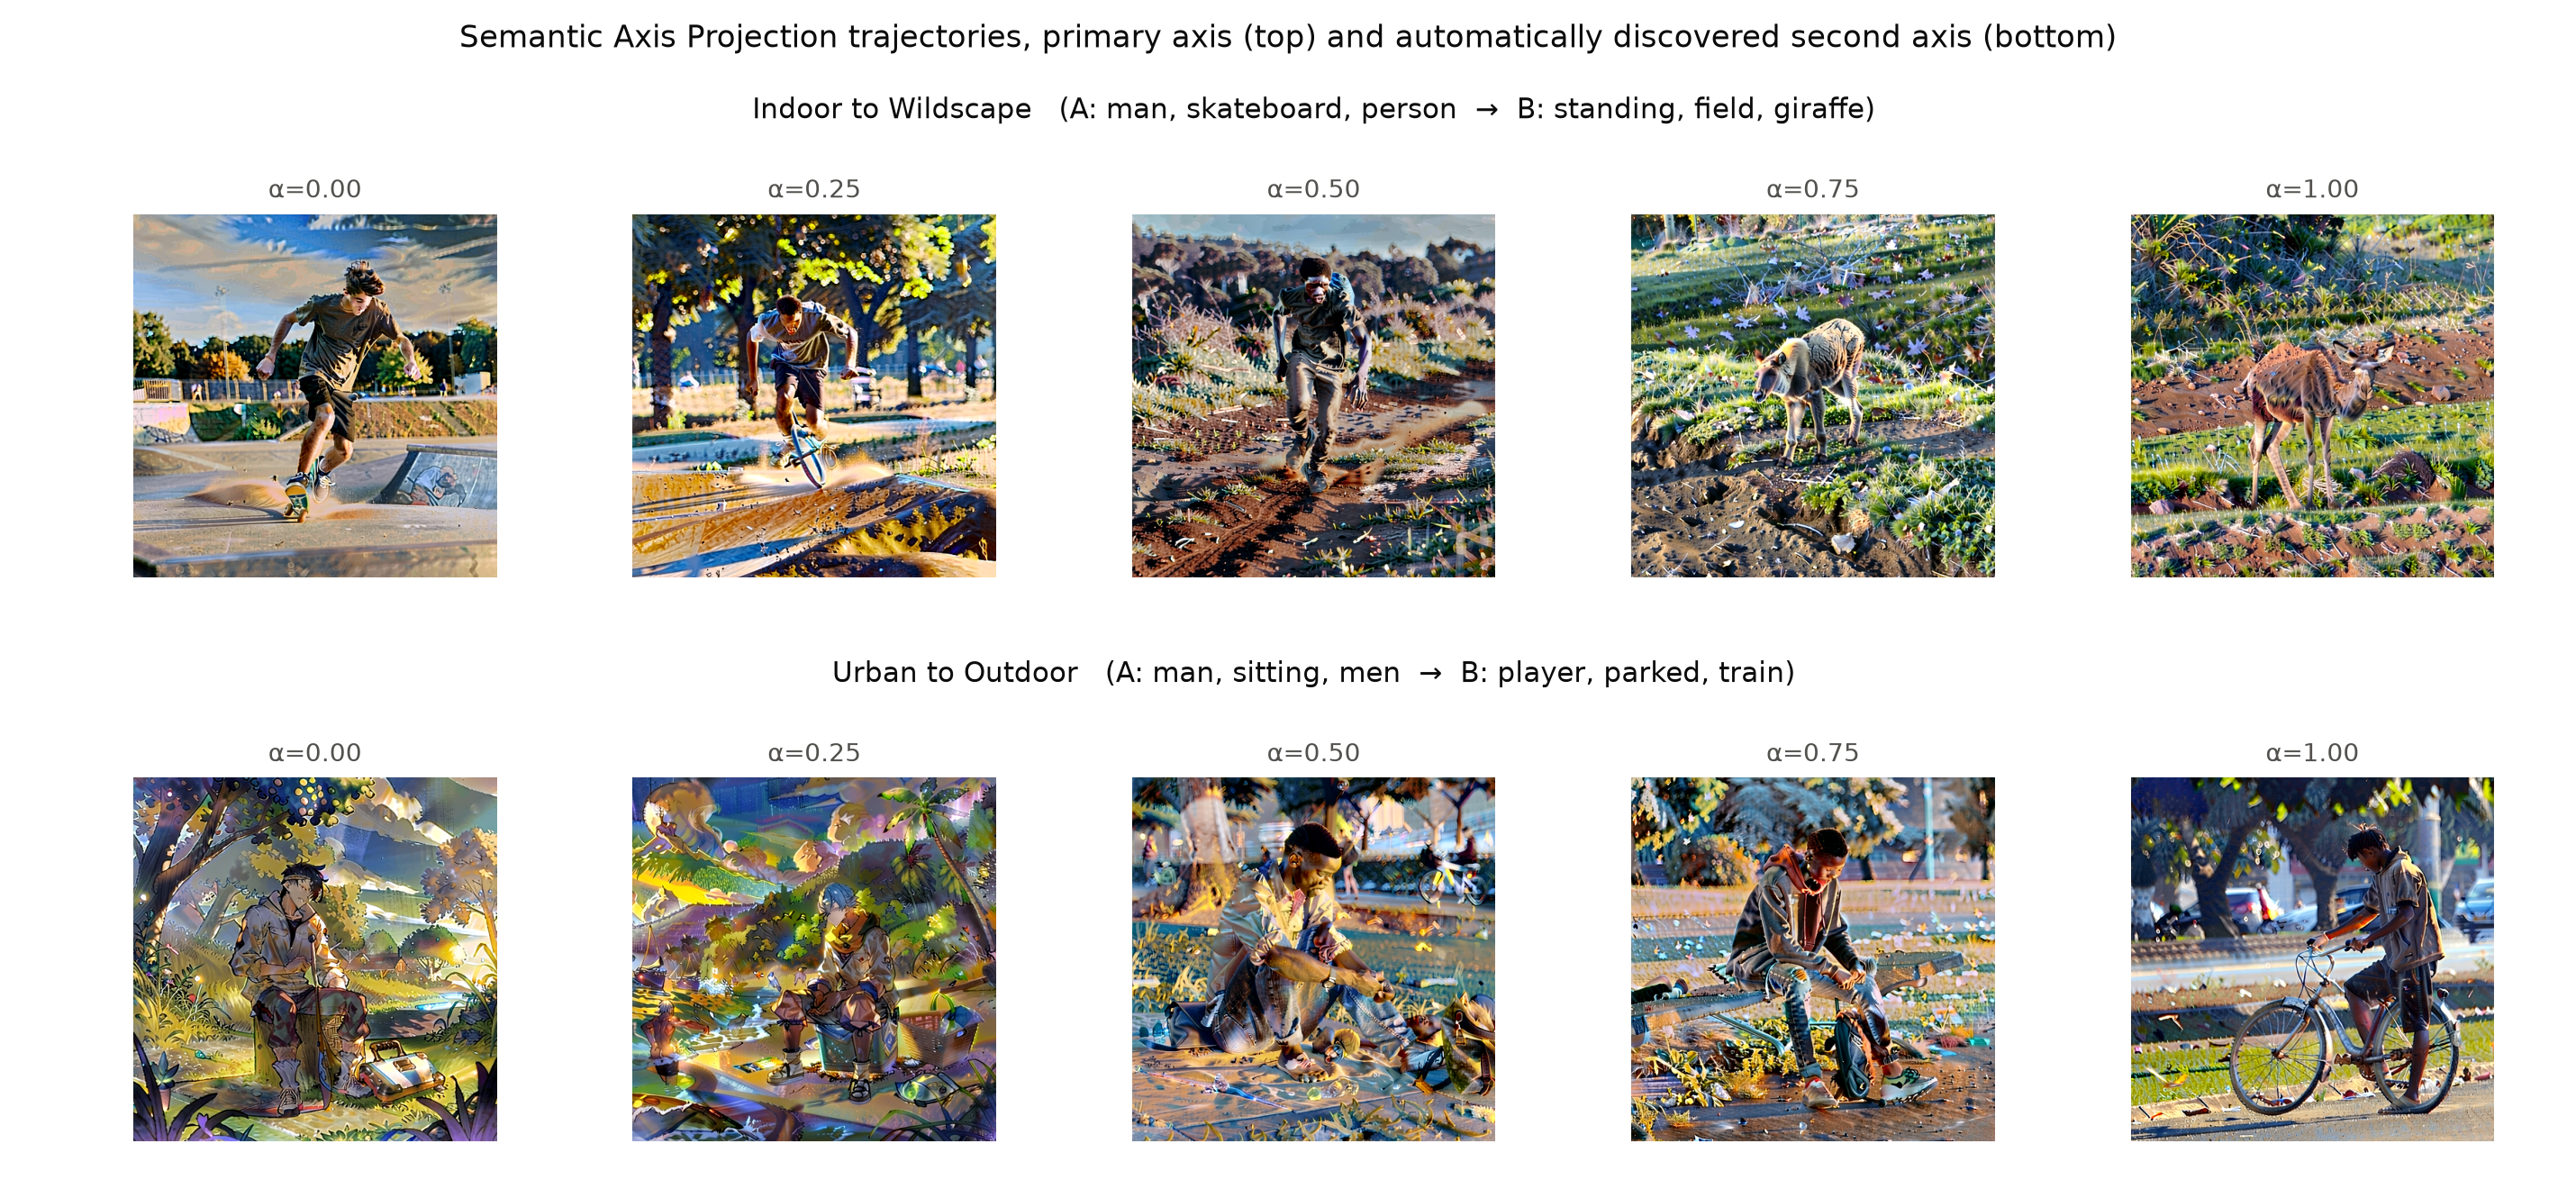
\includegraphics[width=\textwidth]{figures/semantic-axis-projection-generated-images.png}
\caption{Images generated along the primary axis and the automatically discovered second axis with the LLM-generated axis labels and the three contrastive axis terms}
\label{fig:semantic-axis-projection-generated-images}
\end{figure}

\paragraph{Consistency Check:} Consistency Check examines whether small textual changes preserve the position and cluster of a prompt in the compact embedding space. It starts from one selected dataset point and generates several variants of its prompt. The operation then measures how far these variants move away from the original prompt relative to the local scale of the saved dataset. It is therefore an operational test of semantic stability: variants that are intended to remain close in meaning should also remain close to the base prompt in the compact representation.

The operation requires exactly one selected point and an active connection to a CLIP model. It uses the complete original prompt associated with the selected point as the base prompt. The user can configure both the number of generated variants and the variation strength. The number of variants can range from 3 to 20, with a default value of 5, while the variation strength is restricted to the interval from 0.05 to 1.0 and defaults to 0.3.
Reproducibility is ensured by the random seed configured in the NELS Dataset Loader node and is passed down the pipeline into the operation. This seed controls the stochastic components of the operation, including the words selected by the word-dropout procedure and the points sampled from the complete saved dataset as background references for the consistency metric.

For strengths from 0.05 to below 0.35, the operation generates prompt variants using the mentioned word dropout method. If the base prompt contains at least two words, the number of words to remove is calculated as follows:

\texttt{max(1, min(number\_of\_words - 1, round(min(strength, 0.2) * number\_of\_words)))}

The strength-dependent term is capped at 0.2, meaning that the procedure generally removes no more than 20 percent of the words. The value is further limited to keep at least one word in the variant. Finally, the outer max operation guarantees that at least one word is removed, even if rounding would otherwise produce zero. For very short prompts, this minimum removal of one word may therefore exceed the nominal 20 percent limit.
Each accepted candidate must differ from the base prompt, retain at least one word, and be distinct from all previously accepted candidates. To generate the requested number of variants, the operation evaluates up to 8 times as many candidates as requested. Candidates are added in the order in which they are generated, and the procedure terminates once the requested number of distinct valid variants has been obtained. For example, when 5 variants are requested, Consistency Check retains the first 5 candidates that satisfy these conditions. If the procedure cannot generate enough distinct candidates, the remaining result slots are filled with unchanged copies of the base prompt. Word dropout also serves as a fallback if the LLM-based generation path fails. In this fallback mode, the retained words are additionally shuffled when the variation strength exceeds 0.55.

For strengths of 0.35 or higher, the operation instead requests one LLM paraphrase per desired variant. The instruction changes with the selected strength: values below 0.4 request minor rewording and synonyms only, values from 0.4 to below 0.7 request moderate rephrasing with varied structure, and values of 0.7 or above request substantial changes in phrasing. Each call requests the paraphrased prompt as a single plain-text line and is informed of paraphrases that are already accepted, so that repetitions can be avoided. To keep the variants comparable to the complete base prompt, a paraphrase may contain at most five words more than the base prompt. The response budget of the LLM is derived from this limit, combined with an allowance of 3 tokens per permitted word and a minimum of 24 tokens. Word-dropout variants already satisfy the same upper bound because they can only remove or reorder words. If the LLM produces fewer acceptable distinct paraphrases than requested, Consistency Check also fills the remaining result slots with unchanged copies of the base prompt. An example run and its resulting outputs are shown in \hyperref[tbl:consistency-check-variant-examples]{Table~\ref*{tbl:consistency-check-variant-examples}}. The system-prompt template used for LLM paraphrasing, including the strength-dependent style clause, the maximum-word-count rule, and the list of previously accepted paraphrases, is provided in \hyperref[app:3-consistency-check]{Appendix 3}.

\begin{table}[htbp]
\centering
\caption[Consistency Check variants for the shared base prompt (imagenet1k\_labels\_classic), three returned variants per representative strength setting]{Consistency Check variants for the shared base prompt "a photo of great white shark, white shark, man-eater, man-eating shark, Carcharodon carcharias" (\texttt{imagenet1k\_labels\_classic}), three returned variants per representative strength setting}
\label{tbl:consistency-check-variant-examples}
\small
\begin{tabular}{|p{2.1cm}|p{3.4cm}|p{9.2cm}|}
\hline
\textbf{Variation strength} & \textbf{Generation\newline strategy} & \textbf{Variants generated from the shared base prompt} \\
\hline
0.20 & Word dropout & "of great white shark, white shark, man-eater, man-eating Carcharodon carcharias"\newline "a photo of shark, white shark, man-eater, man-eating shark, carcharias"\newline "a white shark, white shark, man-eater, man-eating shark, Carcharodon carcharias" \\
\hline
0.35 & LLM: minor rewording and synonyms & "image of great white shark, white shark, man-eater, Carcharodon carcharias"\newline "picture of great white shark, white shark, predator, Carcharodon carcharias"\newline "snapshot of great white shark, white shark, predator, Carcharodon carcharias" \\
\hline
0.50 & LLM: moderate rephrasing with varied structure & "great white shark image, man-eater, Carcharodon carcharias"\newline "great white shark image, white shark, man-eater predator"\newline "a photo of great white shark, white shark, man-eater, man-eating shark, Carcharodon carcharias" (unchanged base prompt, fallback) \\
\hline
0.80 & LLM: substantial changes in phrasing & "mighty white shark, fierce predator, man's fiercest foe"\newline "mighty white shark, apex predator, human hunter"\newline "vision of mighty white shark, apex predator, human meal, deadly Carcharodon carcharias" \\
\hline
\end{tabular}
\end{table}

The base prompt and all variants are encoded together in one CLIP pass. For every text, this produces real conditioning, a compact embedding, and, when supplied by the encoder, a pooled output. The operation reuses these values for every later stage: the consistency metric, cluster assignment, graph overlay and trajectory construction.

To turn this idea into a comparable result, Consistency Check measures each variant's compact-embedding drift relative to a reference sample drawn from the whole saved dataset. The consistency metric is computed only from the compact embeddings. As in the nearest-neighbor operation, cosine similarity is used. For every variant, its drift from the base prompt is
\[
\mathrm{intra}_i = 1 - \operatorname{cosine}(\mathrm{base}, \mathrm{variant}_i).
\]
Averaging these values yields \texttt{mean intra}, the mean within-set drift. To place this value in context, the operation loads the complete saved compact-embedding matrix for the dataset directly from disk, and samples up to 100 embeddings from it using the dataset loader's random seed. Following this, the same distance metric reference from the base prompt to these samples is computed. Their average, \texttt{mean inter}, is the background reference scale. The final score is
\[
\text{consistency score} = \frac{\text{mean intra}}{\max(\text{mean inter}, \epsilon)},
\]
where $\epsilon$ prevents division by zero. A lower score indicates that the generated variants stayed close to the base prompt relative to this background scale, and a higher score indicates greater relative drift in the model's learned representation. In conclusion, the score is a relative stability measure rather than a universal semantic distance metric, independent of which subset happens to be loaded into the graph panel at the time.

To complement the consistency score with a structural view of the embedding space, Consistency Check assigns each generated variant to a cluster through the dataset's saved runtime cluster-prediction mechanism described in \hyperref[sec:4.6]{Section~4.6}. If the variant is classified as noise, no cluster identifier is reported. This shows whether variants that remain close to the base prompt according to CLIP-space similarity also retain its local cluster context.

Taken together, the result reports for every variant its generated text, its cosine similarity to the base prompt, and the predicted cluster identifier. The graph overlay projects the compact embeddings of the variants through the saved display models. The separate returned trajectory includes the base prompt as its first state, followed by every generated variant. Accordingly, the downstream image-generation node can render the base prompt and all retained variants directly from their attached conditioning, following the common trajectory handoff described at the beginning of this section. A representative rendered example is shown in \hyperref[sec:5.6]{Section~5.6}.

\paragraph{Latent Probe:} Latent Probe reverses the usual direction of the graph exploration. The other operations begin with one or more existing prompts and examine their position, neighborhood, or trajectory in the graph. Latent Probe begins with a position in the graph and asks which prompt representation could plausibly correspond to that location. Its purpose is to investigate whether local geometry in the projected embedding space carries usable semantic information about the underlying prompt representations.

Existing work investigates semantic directions in text embeddings and local geometric structure in diffusion representations, but does not establish a unique or exact mapping from a low-dimensional projection coordinate back to one prompt \cite{yu2024textembedding,park2023riemannian,kwon2023semantic}. NELS therefore treats Latent Probe as an exploratory prototype that serves as an approximation for geometric structure and its semantic encoding. It does not claim to recover an original prompt from a graph coordinate exactly.

The operation has two independent phases: first estimating a compact target vector for the clicked position and, optionally, second reconstructing a prompt near that target. The user chooses whether to place the probe in the 2D or 3D graph view and whether to enable text reconstruction. When reconstruction is enabled, the user can configure the number of seed, noise, and negative examples, as well as the maximum search time and number of refinement iterations that guide the operation.

The frontend first converts the clicked position from the [-1, 1] display space back into raw UMAP coordinates using the inverse of the mapping in \hyperref[sec:4.7]{Section~4.7}. The backend therefore always receives and processes raw 2D or 3D UMAP projection coordinates. It then loads the complete saved reference-coordinate array for the selected UMAP view (\texttt{umap\_2d.npy} or \texttt{umap\_3d.npy}), rather than only the currently loaded subset, together with the memory-mapped compact-embedding matrix (\texttt{compact\_embeddings.npy}). From that data it computes the Euclidean distance from the clicked position to every saved reference coordinate. This is appropriate at this stage because the query and reference points both lie in the same low-dimensional UMAP coordinate system. Thus, the 10 nearest reference points are retained and their compact embeddings are combined into one estimate with inverse-distance weights
\[
w_i = \frac{1}{\mathrm{dist}_i + \epsilon},
\]
normalized so that $\sum_i w_i = 1$. The estimated target vector is then
\[
q = \sum_i w_i \, \mathrm{compact\_embedding}_i.
\]
Here, $\epsilon$ is a small positive constant that prevents division by zero when the clicked position coincides exactly with a saved reference coordinate. Selecting 10 neighbours provides sufficient local coverage for a stable weighted estimate while limiting the influence of points from more distant regions of the projection. Using only one neighbor would make the estimate more sensitive to local projection artifacts, whereas using a substantially larger neighborhood could average away the local structure that the probe is intended to examine. As a result, q is a locally weighted estimate in the compact embedding space. It serves as the target for nearest-prompt retrieval, approximate cluster assignment, and optional text reconstruction.

The estimated vector \texttt{q} is passed to the dataset's cluster-prediction mechanism described in \hyperref[sec:4.6]{Section~4.6}. The resulting cluster id, noise flag, and membership strength are approximate runtime assignments. Latent Probe also compares \texttt{q} with the compact tensors of the currently loaded points using cosine similarity and returns up to the requested number of nearest existing prompts, defaulting to 15 when no request is defined. Each hit contains an id, a similarity score, the full prompt text, and a display label capped at 80 characters. The graph panel displays up to the five highest-scoring prompts from this result set. If no points are loaded, or none carries a usable tensor, the same lookup falls back to the complete saved dataset and reads only the necessary rows from \texttt{samples.jsonl}. Such fallback hits may not correspond to points currently rendered on the canvas and are therefore not necessarily clickable in the graph panel.

Text reconstruction runs only when it is enabled and the probe lookup produced at least one usable hit. Its objective is to find a new prompt whose embedding lies close to q. First, the reconstruction context is assembled from the currently loaded subset. The retrieved nearest prompts described above serve as positive seed examples for the LLM-based search. The least similar loaded points are used as negative examples that define concepts to avoid. Additional points are sampled from the middle of the similarity ranking as noise examples. Building on this, the initial LLM call seeds and noise texts are combined as positive examples near the target, while negative texts specify, as mentioned above, themes to avoid. The result also returns the identifiers and truncated labels of all three categories as an inspectable record of the context supplied to the first LLM call. If the LLM produces no valid initial candidate, the lookup and cluster result remain available, but no reconstruction trajectory is created.

With the explained reconstruction context above, reconstruction begins with an LLM prompt that requests up to 16 new, self-contained image descriptions of 5 to 20 words. The generated descriptions must not copy phrases from the reference prompts. Each candidate is re-encoded with CLIP, converted into a compact embedding, and scored by cosine similarity to q. The eight highest-scoring candidates form the initial beam.
In each subsequent round, the LLM receives this ranked beam, including the current similarity scores, together with the negative examples. It proposes up to 16 refinements, which get combined with the previous beam while removing duplicate prompt texts. Finally eight best candidates are retained. During each completed search step, the graph panel receives a WebSocket progress event containing the current best prompt and its similarity score. Finally, the search stops when it reaches the configured time or iteration limit, when the LLM produces no new candidate, or when the best score fails to improve by more than 0.0007 for four consecutive rounds. To summarize, the reconstruction is trying to match the estimated target vector q in the compact embedding space, to be able to approximate a prompt for the clicked position in the UMAP projection.

The two LLM instruction templates used for the initial candidate generation and the later refinement rounds are provided in \hyperref[app:3-latent-probe]{Appendix 3}.

The resulting trajectory is a compact record of the search progress. Once valid initial candidates exist, Latent Probe always records the first beam state. A later state is recorded only when its best score exceeds that of the preceding snapshot by more than 0.0001. The final state is retained in every case. If its best prompt matches the last recorded prompt, the operation updates that snapshot instead of adding a duplicate. Otherwise, it appends the final state as a new snapshot.
Each recorded state contains its final compact tensor and real CLIP conditioning. If the connected encoder provides a pooled output, this value is stored as well. No additional conditioning step is required before image generation. Its associated texts are the prompts generated during the search, and each trajectory step refers to one prompt by its position in that ordered list. Accordingly, the downstream image-generation node can render the recorded states directly from their attached conditioning, following the common trajectory handoff. An example search and its retained snapshots are shown in \hyperref[fig:latent-probe-generated-images]{Figure~\ref*{fig:latent-probe-generated-images}}.

\begin{figure}[htbp]
\centering
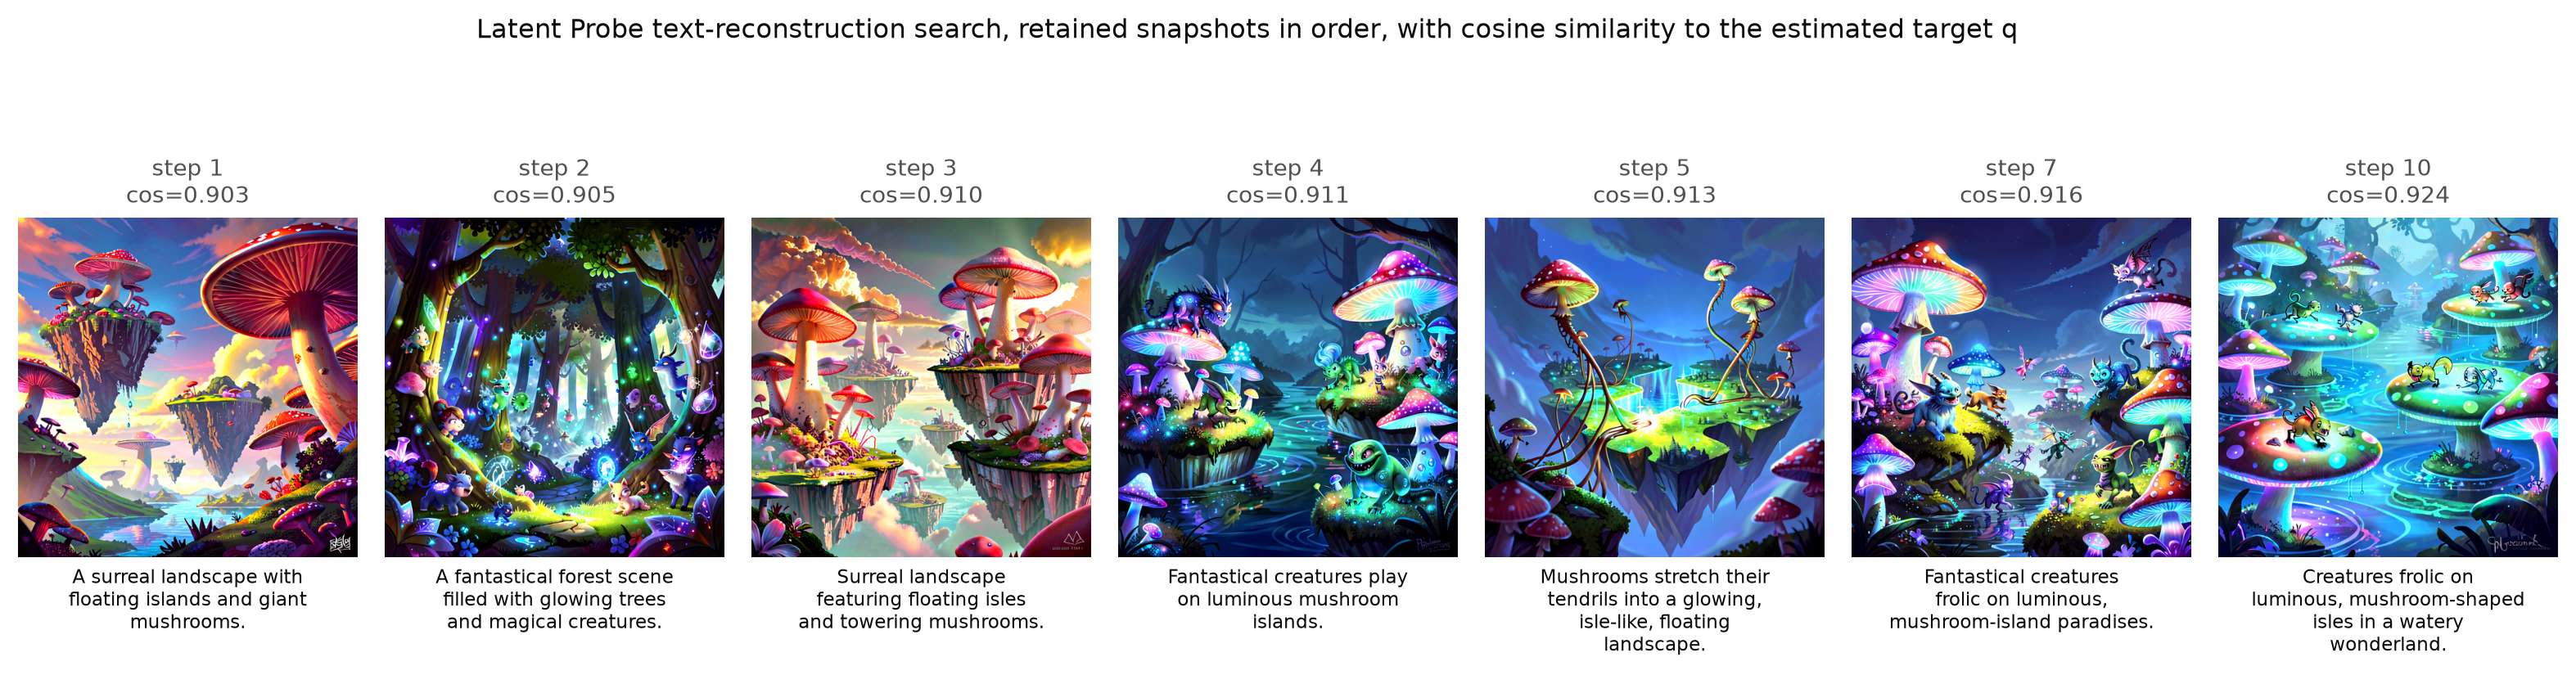
\includegraphics[width=\textwidth]{figures/latent-probe-generated-images.png}
\caption{Latent Probe text-reconstruction search, retained snapshots in order, with cosine similarity to the estimated target q and the reconstructed prompt text below each image}
\label{fig:latent-probe-generated-images}
\end{figure}

\section{Design tradeoffs and validity limits}\label{sec:4.9}

Several limitations arise directly from the design decisions presented in this chapter rather than from implementation errors. The system uses compact embeddings for analysis and navigation, while image generation relies on the original conditioning tensors. This separation keeps the panel responsive and preserves compatibility with the KSampler (ComfyUI's diffusion-sampling node), but it also means that proximity in the graph does not necessarily correspond to proximity in the conditioning space used for generation. Consequently, a point that appears close to its neighbors on the canvas may still differ substantially from them in the full conditioning representation. Moreover, compact embeddings are inherently lossy. Regardless of the pooling method used to create them (\hyperref[sec:4.6]{Section~4.6}), token-level information is reduced to a single fixed-size vector, which may conceal subtle semantic differences that remain present in the complete sequence tensor.

UMAP, HDBSCAN, and the inverse estimation applied by Latent Probe are approximate methods rather than exact geometric procedures. Their projected distances, cluster boundaries, and estimated target embeddings should therefore be interpreted as practical approximations rather than exact results.

Dataset construction introduces additional scalability limitations. Prompt encoding is performed sequentially, requiring one forward pass per prompt because pooled outputs are obtained individually. Furthermore, fitting UMAP and HDBSCAN is CPU-bound. As described in \hyperref[sec:4.6]{Section~4.6}, adding new prompts requires the projection and clustering models to be refitted on the complete dataset rather than updated incrementally. Consequently, extending an existing dataset remains computationally expensive.

The \texttt{classic} strategy was the preferred approach for the large-scale operation datasets, since it reuses the canonical fit directly rather than introducing a separate runtime approximation, and later proved to be the most accurate of the three strategies at reproducing the canonical fit (\hyperref[sec:5.2]{Section~5.2}). It was nevertheless not used for the four large-scale operation datasets described in \hyperref[sec:4.5]{Section~4.5}. An exploratory \texttt{classic} build at the target size of 550.000 prompts showed that each of the three serialized runtime UMAP models (cluster space, 2D, and 3D) reached approximately 50 GB, since the underlying UMAP implementation stores a copy of the training data together with its nearest-neighbor search index as attributes of the fitted model object, all of which are serialized into the same file when the model is persisted. Loading and holding three such models simultaneously is not feasible on typical consumer hardware, which motivated the use of the \texttt{two\_pass} strategy's smaller, subset-trained runtime models for the large-scale datasets instead.

The \texttt{parametric} projection strategy introduces further dependencies and training overhead through Parametric UMAP and TensorFlow. Its current implementation is not yet fully robust for very large embedding matrices, where fitting may fail because of resource constraints. For this reason, the four large-scale operation datasets described in \hyperref[sec:4.5]{Section~4.5} use the \texttt{two\_pass} strategy, while \texttt{parametric} is applied only to the smaller ImageNet-1k comparison dataset. Two concrete instances of this robustness limitation were investigated in more detail below, namely a reproducibility failure at the ImageNet-1k scale, and a hard scalability failure at a substantially larger corpus size.

This reproducibility limitation was examined by rebuilding the \texttt{parametric} ImageNet-1k comparison dataset using the same input data, parameters, random seed, and library versions. Despite these identical conditions, the resulting clustering differed substantially. The divergence was traced to non-deterministic floating-point behavior during TensorFlow CPU training with oneDNN acceleration, where small numerical differences accumulated over training and produced different network parameters. After disabling oneDNN through the \texttt{TF\_ENABLE\_ONEDNN\_OPTS} setting, repeated runs produced bit-identical outputs.

A more severe scalability failure occurred when constructing a \texttt{parametric} dataset from approximately 61.700 prompts. Training terminated before producing a projection because the serialized TensorFlow computation graph exceeded protobuf's fixed 2 GB message-size limit. This restriction originates within the TensorFlow, Keras, and \texttt{umap-learn} stack rather than in the NELS implementation itself. Since the failure occurred at approximately one ninth of the size of the large operation datasets used in this thesis, it further supports the use of the \texttt{two\_pass} strategy instead of \texttt{parametric} for large-scale datasets.

These design trade-offs and validity limitations establish the scope within which the implementation can be evaluated. \hyperref[ch:results]{Chapter~5} presents this empirical evaluation and examines how the operations introduced in this chapter behave in practice.
